\documentclass[tese_patricia]{subfiles}% !TeX spellcheck = pt_BR

\begin{document}
\nomenclature[B,01]{$\domainT$}{Domínio computacional de um escoamento em um instante de tempo arbitrário $t$;}
\nomenclature[B,02]{$n_{sd}$}{Dimensão espacial;}
%\nomenclature[B,03]{$\boundaryT$}{Contorno do domínio computacional de um escoamento em um instante de tempo arbitrário $t$;}
%\nomenclature[B,04]{$t$}{Instante de tempo arbitrário;}
%\nomenclature[B,05]{$\totalTime$}{Intervalo de tempo total da análise;}
%\nomenclature[B,06]{$\density$}{Massa específica do fluido;}
%\nomenclature[B,07]{$\velocity$}{Campo de velocidades de um escoamento;}
%\nomenclature[B,08]{$\sbodyforce$}{Força de domínio em um escoamento;}
%\nomenclature[B,09]{$\stresstensor$}{Tensor das tensões de Cauchy;}
%\nomenclature[B,10]{$\press$}{Campo de pressões de um escoamento;}
%\nomenclature[B,11]{$\viscosity$}{Viscosidade dinâmica do fluido;}
%\nomenclature[B,12]{$\strainratetensor(\bullet)$}{Tensor taxa de deformação de um campo escalar ou vetorial;}
%\nomenclature[B,13]{$\mathbf{g}$}{Condições de contorno de Dirichlet;}
%\nomenclature[B,14]{$\mathbf{h}$}{Condições de contorno de Neumann;}
%\nomenclature[B,15]{$\left(\boundaryT\right)_{\mathbf{g}$}}{Porção do contorno com condições de contorno de Dirichlet;}
%\nomenclature[B,16]{$\left(\boundaryT\right)_{\mathbf{h}$}}{Porção do contorno com condições de contorno de Neumann;}
%\nomenclature[B,17]{$\normal$}{Vetor normal ao contorno do domínio computacional;}
%\nomenclature[B,18]{$\Omega_X$}{Domínio computacional inicial ou material;}
%\nomenclature[B,19]{$\mathbf{X}$}{Coordenadas no domínio inicial ou material de um ponto arbitrário;}
%\nomenclature[B,20]{$\Omega_x$}{Domínio computacional atual;}
%\nomenclature[B,21]{$\pos$}{Coordenadas atuais de um ponto arbitrário;}
%\nomenclature[B,22]{$\Omega_{\bar{x}}$}{Domínio computacional de referência;}
%\nomenclature[B,23]{$\posAle$}{Coordenadas de referência de um ponto arbitrário;}
%\nomenclature[B,24]{${\mathbf{\Phi}}$}{Função mudança de configuração do domínio computacional material para o domínio computacional atual;}
%\nomenclature[B,25]{$\bar{\mathbf{\Phi}}$}{Função mudança de configuração do domínio computacional de referência para o domínio computacional atual;}
%\nomenclature[B,26]{$\velocityALE$}{Velocidade dos pontos de referência;}
%\nomenclature[B,27]{$\usolution$}{Espaço vetorial das funções aproximadoras do campo de velocidades;}
%\nomenclature[B,28]{$\psolution$}{Espaço vetorial das funções aproximadoras do campo de pressões;}
%\nomenclature[B,29]{$\uweighting$}{Espaço vetorial das funções ponderadoras do campo de velocidades;}
%\nomenclature[B,30]{$\pweighting$}{Espaço vetorial das funções ponderadoras do campo de pressões;}
%\nomenclature[B,31]{$\utest$}{Função ponderadora pertencente ao espaço $\uweighting$;}
%\nomenclature[B,32]{$\ptest$}{Função ponderadora pertencente ao espaço $\pweighting$;}
%\nomenclature[B,33]{$(\bullet)^h$}{O superscrito $h$ indica, em todos os casos, a discretização em elementos finitos da variável;}
%\nomenclature[B,34]{$\domain^{e}$}{Domínio computacional de um elemento finito;}
%\nomenclature[B,35]{$\nel$}{Número de subdomínios do domínio discreto;}
%\nomenclature[B,36]{$N_nos$}{Número de nós ou pontos de controle do domínio discreto;}
%\nomenclature[B,37]{$N$}{Função de forma da discretização do domínio;}
%\nomenclature[B,38]{$(\bullet)_A$}{O subscrito $A$ indica, em todos os casos, que se trata da variável respectiva ao nó $A$ da malha de elementos finitos;}
%\nomenclature[B,39]{$\SUPG$}{Parâmetro de estabilização do método \textit{Streamline-Upwind/Petrov-Galerkin} (SUPG);}
%\nomenclature[B,40]{$\PSPG$}{Parâmetro de estabilização do método \textit{Pressure-Stabilizing/Petrov-Galerkin} (PSPG);}
%\nomenclature[B,41]{$\LSIC$}{Parâmetro de estabilização do método \textit{Least-Squares on the Incompressibility Constraint} (LSIC);}
%\nomenclature[B,42]{$\resMom$}{Resíduo da equação da quantidade de movimento;}
%\nomenclature[B,43]{$\resPre$}{Resíduo da equação da continuidade;}
%\nomenclature[B,44]{$\NNSM$}{Resíduo do vetor discreto da equação da quantidade de movimento;}
%\nomenclature[B,45]{$\NNSC$}{Resíduo do vetor discreto da equação da continuidade;}
%\nomenclature[B,46]{$\Acceleration$}{Vetor nodal dos graus de liberdade respectivo a aceleração;}
%\nomenclature[B,47]{$\Velocity$}{Vetor nodal dos graus de liberdade respectivo a velocidade;}
%\nomenclature[B,48]{$\Press$}{Vetor nodal dos graus de liberdade respectivo a pressão;}
%\nomenclature[B,49]{$\matrixQ$}{Tensor métrico do elemento;}
%\nomenclature[B,50]{$\coordAdimen$}{Coordenadas adimensionais do elemento onde são definidas as funções de forma;}
%\nomenclature[B,51]{$\matrixD$}{Matriz que escalona o tensor métrico do elemento;}
%\nomenclature[B,52]{$\matrixQhat$}{Tensor métrico do elemento escalonado;}
%\nomenclature[B,53]{$\bar{\coordAdimen}$}{Coordenadas adimensionais do espaço preferido;}
%\nomenclature[B,54]{$\mathbf{C}$}{Tensor de transformação de Bezier;}
%\nomenclature[B,55]{$\RGN$}{Comprimento de escala do elemento finito;}
%\nomenclature[B,56]{$\rRGN$}{Vetor unitário no sentido da velocidade do fluido no elemento finito;}
%\nomenclature[B,57]{$\matrixG$}{Matriz auxiliar para o cálculo do comprimento direcional do elemento;}
%\nomenclature[B,58]{$h_{min}$}{Mínimo comprimento de escala do elemento finito;}
%\nomenclature[B,59]{$h_{max}$}{Máximo comprimento de escala do elemento finito;}
%\nomenclature[B,60]{$\SUGNi,\SUGNii,\SUGNiii$}{Parâmetros da estabilização SUPG/PSPG/LSIC correspondentes aos termos convectivos, inerciais e viscosos, respectivamente;}
%\nomenclature[B,61]{$\timeStep$}{sub-intervalo de tempo $t$;}
%\nomenclature[B,62]{$\rRGN_{reg}$}{Vetor unitário no sentido da velocidade do fluido modificado de maneira a evitar problemas numéricos devido divisão por zero;}
%\nomenclature[B,63]{$\varepsilon$}{Constante pequena utilizada no cálculo de $\rRGN_{reg}$;}
%\nomenclature[B,64]{$t_{n}$}{extremidade menor de tempo do sub-intervalo $\timeStep$;}
%\nomenclature[B,65]{$t_{n+1}$}{extremidade maior de tempo do sub-intervalo $\timeStep$;}
%\nomenclature[B,66]{$\alpham, \alphaf, \gamma$}{Parâmetros reais do esquema de integração temporal $\alpha$-generalizado;}
%\nomenclature[B,67]{$\specRadius$}{Raio espectral da matriz de amplificação;}
%\nomenclature[B,68]{$\Reynolds$}{Número de Reynolds;}
%\nomenclature[B,69]{$\velocinfty$}{Velocidade de referência;}
%\nomenclature[B,70]{$L$}{Comprimento característico/de referência do escoamento;}
%\nomenclature[B,71]{$\kviscosity$}{Viscosidade cinemática do fluido;}
%\nomenclature[B,72]{$u_x$}{Velocidade do escoamento na direção $x$;}
%\nomenclature[B,73]{$u_y$}{Velocidade do escoamento na direção $y$;}
%\nomenclature[B,74]{$u_n$}{Velocidade do escoamento na direção normal ao contorno;}
%\nomenclature[B,75]{$F_L, F_D$}{Forças de sustentação e arrasto, respectivamente;}
%\nomenclature[B,76]{$C_L, C_D$}{Coeficiente de sustentação e arrasto, respectivamente;}
%\nomenclature[B,77]{$\Strouhal$}{Número de Strouhal;}
%\nomenclature[B,78]{$f_V$}{Frequência de desprendimento dos vórtices;}

% ---------------------------------------------------------- 
% Métodos de \part{\part{malhas}} sobrepostas
% ----------------------------------------------------------
\chapter[Dinâmica dos fluidos computacional]{Dinâmica dos fluidos computacional}
\label{capitulo:Cap2}
% ----------------------------------------------------------

O escoamento isotérmico de um fluido newtoniano é governado pelas equações advindas da conservação da quantidade de movimento, ou de Navier-Stokes, e da conservação de massa. Nos casos em que ocorram variações significativas no campo de temperatura, ou em escoamentos compressíveis, a equação da conservação de energia deve ser adicionada ao sistema. Essas equações governantes, juntamente com as relações constitutivas, resultam em um sistema de equações diferenciais não lineares que descrevem o comportamento do escoamento no tempo e no espaço. 

Neste trabalho são analisados escoamentos incompressíveis isotérmicos e com contornos móveis. Nas próximas seções, são apresentadas as principais técnicas utilizadas na solução desse tipo de problema e sua implementação computacional. Uma descrição Euleriana-Lagrangiana arbitrária é utilizada para as equações e a discretização espacial se dá através da método dos elementos finitos (FEM) ou da análise isogeométrica (IGA). Para resolver os problemas numéricos típicos desse sistema de equações, como as oscilações espúrias que ocorrem em problemas com convecção dominante quando aplicado o método dos resíduos ponderados baseado na técnica de Galerkin clássica, a metodologia SUPG é utilizada. Além disso, para contornar a restrição de \textit{Ladyzhenskaya-Babuška-Brezzi} ou LBB a técnica de estabilização PSPG é aplicada. A integração temporal das equações é realizada pelo método $\alpha$-generalizado. No final deste capítulo, apresenta-se um algoritmo que descreve o esquema de solução computacional dos problemas da DFC seguido da solução de alguns problemas clássicos da DFC para sua verificação.

\section{Forma forte das equações governantes} 

As equações de Navier-Stokes são derivadas da segunda lei de Newton, e são obtidas através do balanço entre a resultante das forças externas que atuam em um elemento infinitesimal de fluido e a sua variação temporal da quantidade de movimento, resultando:

\begin{align}
\density\left(\frac{\partial\velocity}{\partial t} + \velocity\cdot\nabla\velocity - \externalforce \right) - \nabla \cdot \stresstensor &= \mathbf{0} , \label{eq:Navier-Stokes} 
\end{align}

\noindent onde $\density$, $\velocity$ e $\externalforce$ são respectivamente a densidade, a velocidade e a forças de domínio por unidade de massa. O tensor de tensões de Cauchy $\stresstensor$ é definido para fluidos newtonianos incompressíveis pela seguinte relação constitutiva:

\begin{align}
\stresstensor &= -p\unittensor + 2\viscosity\strainratetensor(\velocity),\label{eq:StressTensor}
\end{align}

\noindent onde $p$ representa a pressão, $\viscosity$ a viscosidade dinâmica do fluido e $\strainratetensor$ é o tensor taxa de deformação, definido como:

VER SOBRE A DEFINIÇÃO DE TAXA LÁ NO CAPÍTULO 6

\begin{align}
\strainratetensor\left(\velocity\right) = \frac{1}{2}\left(\nabla\left(\velocity\right) + \nabla\left(\velocity\right)^{T}\right). 
\label{eq:StrainTensor}
\end{align}

A equação de conservação da massa realiza um balanço em um volume de controle infinitesimal entre as parcelas de massa que entram e saem por unidade de tempo, definindo a variação da densidade. Para um escoamento incompressível a variação da densidade é nula, de modo que a equação se resume a:

\begin{align}
\nabla \cdot \velocity &= 0. 
\end{align}

As condições de contorno essenciais, ou de Dirichlet, e as condições de contorno naturais, ou de Neumann, são necessárias para completar as equações da mecânica dos fluidos, e são descritas respectivamente por:

\begin{align}
\velocity = \mathbf{g} \textrm { em} \left(\boundaryT\right)_{\mathbf{g}} \label{eq:Dir},\\
\stresstensor \cdot \snormal = \mathbf{h} \textrm{ em} \left(\boundaryT\right)_{\mathbf{h}}, \label{eq:Neu}
\end{align}

\noindent sendo $\left(\boundaryT\right)_{\mathbf{g}}$ a porção do contorno com condições de contorno de Dirichlet, representadas pelo vetor $\mathbf{g}$, e $\left(\boundaryT\right)_{h}$ aquela com condições de contorno de Neumann, descritas por $\mathbf{h}$. A variável $\snormal$ representa o vetor unitário normal ao contorno em análise.


\section{Descrição Euleriana-Lagrangiana arbitrária (ALE)} \label{Capítulo2:ALE}

A descrição Lagrangiana-Euleriana arbitrária \cite{DoneaGH:1982} representa uma generalização da descrição puramente Lagrangiana e da descrição puramente Euleriana do movimento do contínuo. A descrição Lagrangiana fixa a atenção em pontos materiais do contínuo, enquanto que na descrição Euleriana considera-se uma porção fixa do espaço ocupada pelo contínuo, e analisam-se os pontos materiais que passam por essa porção ao longo do tempo. Como consequência, na descrição puramente Lagrangiana a malha computacional move-se com o contínuo, enquanto que na Euleriana a malha computacional mantém-se fixa. Por sua vez, na descrição Lagrangiana-Euleriana arbitrária, trabalha-se com pontos de referência que podem movimentar-se, mas de maneira independente do movimento dos pontos materiais do contínuo analisado.

Para a aplicação dessa metodologia às equações governantes da mecânica dos fluidos é importante a definição de três domínios, de acordo com a Fig. \ref{fig:Ale}. O domínio inicial, chamado de \textbf{domínio material} ($\Omega_X$), que é definido pelas coordenadas dos pontos materiais $\mathbf{X}$; O domínio atual, chamado de \textbf{domínio espacial} ($\Omega_x$), definido pelas coordenadas $\pos$; e por fim, o \textbf{domínio de referência} ($\Omega_{\bar{x}}$) com coordenadas dos pontos de referência $\posALE$. 

As coordenadas no domínio atual do contínuo podem ser mapeadas a partir do domínio inicial ou a partir do domínio de referência utilizando as seguintes funções de mapeamento:  

\begin{align}
\pos = \mathbf{\Phi}(\mathbf{X},t) = \bar{\mathbf{\Phi}}(\bar{\mathbf{x}},t). \label{eq:Pos}
\end{align}

\begin{figure}[htb!]
	\centering
	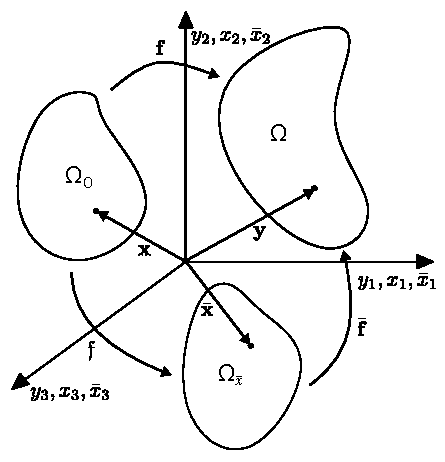
\includegraphics[scale=1.0]{Imagens/Cap2/ALE.pdf}	
	\caption{Domínios utilizados para a descrição Lagrangiana-Euleriana arbitrária}
	\label{fig:Ale}
\end{figure}

\noindent a velocidade, por sua vez, para os pontos materiais ($\velocity$) no instante $t$ é obtida pela derivada do vetor posição $\pos$ mantendo $\mathbf{X}$ fixo:

\begin{align}
\velocity = \left. \frac{\partial\pos\left(\mathbf{X},t\right)}{\partial t} \right|_\mathbf{X}, \label{eq:vel}
\end{align}

\noindent e a velocidade do contínuo nos pontos de referência $\velocityALE$ é descrita como:

\begin{align}
\velocityALE = \left. \frac{\partial\pos\left({\posALE},t\right)}{\partial t} \right| _{\posALE}. \label{eq:velALE}
\end{align}

Para expressar as equações da dinâmica dos fluidos em descrição Lagrangiana-Euleriana arbitrária, parte-se do conceito de \textit{derivada material}. A derivada material de uma propriedade qualquer $F$ do contínuo é definida como a variação por unidade de tempo sentida por um observador movendo-se junto com os pontos materiais e é escrita como $\frac{DF}{Dt}$. A derivada material da velocidade, variável de interesse para as equações da mecânica dos fluídos, quando representada pelo domínio espacial é definida como:

\begin{align}
\frac{D\velocity}{Dt} = \left. \frac{\partial\velocity\left(\pos,t\right)}{\partial t} \right|_\mathbf{x} + \left. \frac{\partial\velocity\left(\pos,t\right)}{\partial \pos} \right|_{t} \left. \frac{\partial\pos}{\partial t} \right|_{\mathbf{X}}. \label{eq:MatDerEulerian}
\end{align}

Aplicando-se a Eq. \eqref{eq:vel} à Eq. \eqref{eq:MatDerEulerian} pode-se reescrevê-la como:

\begin{align}
\frac{D\velocity}{Dt} = \left. \frac{\partial\velocity\left(\pos,t\right)}{\partial t} \right|_\mathbf{x} + \velocity \left. \frac{\partial\velocity\left(\pos,t\right)}{\partial \pos} \right|_{t}. \label{eq:MatDerEulerianUp}
\end{align}

Baseado nessa última expressão as equações de Navier-Stokes para escoamento incompressível podem ser apresentadas, em termo da derivada material, da seguinte forma:

\begin{align}
\density\left(\frac{D\velocity}{Dt} - \externalforce \right) - \nabla \cdot \stresstensor &= \mathbf{0}. \label{Navier-Stokes-MatDerEuleriana}
\end{align}

Utilizando-se agora o domínio de referência $\Omega_{\bar{x}}$, para expressar a derivada material chega-se à seguinte expressão:

\begin{align}
\frac{D\velocity}{Dt} = \left. \frac{\partial\velocity\left(\posALE,t\right)}{\partial t} \right|_{\posALE} + \left. \frac{\partial\velocity\left(\posALE,t\right)}{\partial \posALE} \right|_{t} \left. \frac{\partial\posALE}{\partial t} \right|_{\mathbf{X}}. \label{eq:MatDerALE}
\end{align}
%

Derivando-se \eqref{eq:Pos} no tempo com $\mathbf{X}$ fixo, é possível escrever:

\begin{align}
\left. \frac{\partial \pos}{\partial t} \right|_{\mathbf{X}} = \left . \frac{\partial \mathbf{\Phi}}{\partial t} \right|_{\mathbf{X}} =   \left . \frac{\partial \bar{\mathbf{\Phi}}}{\partial t} \right|_{\posALE} + \left . \frac{\partial \bar{\mathbf{\Phi}}}{\partial \posALE} \right|_{t} \left . \frac{\partial \posALE}{\partial t} \right|_{\mathbf{X}},
\end{align}

\noindent onde o termo $\left. \frac{\partial \bar{\mathbf{\Phi}}}{\partial t} \right|_{\posALE}$ representa a velocidade do domínio de referência (malha de elementos finitos), em relação ao domínio espacial, representada por $\velocityALE$, permitindo escrever: 

\begin{align}
\velocity = \velocityALE + \left . \frac{\partial \pos}{\partial \posALE} \right|_{t} \left . \frac{\partial \posALE}{\partial t} \right|_{\mathbf{X}},
\end{align}

\noindent ou ainda:

\begin{align}
\left . \frac{\partial \posALE}{\partial t} \right|_{\mathbf{X}} = \left( \velocity - \velocityALE \right) \left. \frac{\partial \posALE}{\partial \pos} \right |_{t}. \label{eq:velRel}
 \end{align}
 
Utilizando-se das expressões Eq. \eqref{eq:velRel} e Eq. \eqref{eq:MatDerALE} obtêm-se que: 
 
\begin{align}
\frac{D\velocity}{Dt} = \left. \frac{\partial\velocity\left(\posALE,t\right)}{\partial t} \right|_{\posALE} +  \left( \velocity - \velocityALE \right) \left. \frac{\partial\velocity\left(\posALE,t\right)}{\partial \pos} \right|_{t}. \label{eq:MatDerALEUp}
\end{align}

Por fim, aplicando-se a Eq. \eqref{eq:MatDerALEUp} em Eq. \ref{Navier-Stokes-MatDerEuleriana}, chega-se à equação da conservação da quantidade de movimento para escoamentos incompressíveis em descrição Lagrangiana-Euleriana arbitrária:

\begin{align}
\density \left . \left(\frac{\partial\velocity}{\partial t} \right|_{\posALE} + \left(\velocity - \velocityALE\right)\cdot\nabla\velocity - \externalforce \right) - \nabla \cdot \stresstensor &= \mathbf{0}.  \label{eq:Navier-Stokes-ALE} 
\end{align}

Já para o caso incompressível, a equação da continuidade 

\begin{align}
\nabla \cdot \velocity &= 0 \label{eq:Continuity}
\end{align}

\noindent continua válida para a descrição ALE.


\section{Forma Fraca e discretização espacial} \label{capitulo:Cap2:FormaFraca}

LEMBRAR DE ORGANIZAR PARA DEIXAR COMPATÍVEL COM O QUE FOI ESCRITO NO CAPÍTULO 6.

Tomando-se a forma forte das equações governantes, aplica-se o método de resíduos ponderados para se chegar à forma fraca e proceder com a discretização espacial. Os espaços de dimensão finita das funções tentativa que descrevem a velocidade e a pressão são chamados de $\usolution$ e $\psolution$ respectivamente, e definidos como:

\begin{align}
\usolution = \left\{\velocity \left . \right| \velocity \left(\cdot,t\right) \in \left(H^{1}\left(\domainT\right)\right)^{n_{sd}}, u_{i} = g_{i} \textrm { em} \left(\boundaryT\right)_{g_i} \right\}
\end{align}

\noindent e

\begin{align}
\psolution = \left\{\press \left . \right| \press \left(\cdot\right) \in L^{2}\left(\domainT\right), \int_{\domainT}\press \textrm { } d\domain = 0 \textrm { se } \boundaryT =\left(\boundaryT\right)_{\mathbf{g}} \right\},
\end{align}

\noindent sendo $L^{2}\left(\domainT\right)$ o espaço de funções escalares que são de quadrado integrável sobre $\domainT$; e $\left(H^{1}\left(\domainT\right)\right)^{n_{sd}}$ é o espaço de funções vetoriais com derivadas de quadrado integrável sobre $\domainT$.

O espaço das funções teste ou funções peso das equações da quantidade de movimento e da continuidade são definidos respectivamente por:

\begin{align}
\uweighting = \left\{\utest \left . \right| \utest \left(\cdot\right) \in \left(H^{1}\left(\domainT\right)\right)^{n_{sd}}, w_{i} = 0 \textrm { em} \left(\boundaryT\right)_{g_i} \right\},
\end{align}


\begin{align}
\pweighting = \psolution.
\end{align}

Aplicando-se o método dos resíduos ponderados sobre as equações Eq. \eqref{eq:Navier-Stokes-ALE} e Eq. \eqref{eq:Continuity}, integrando-se por partes o termo referente ao tensor de tensões de Cauchy, empregando-se o teorema da divergência e levando-se em consideração a condição de homogeneidade da função $\utest$ sobre o contorno $\left(\boundaryT\right)_{\mathbf{g}}$, obtém-se a forma fraca. A solução do problema consiste então em encontrar $\velocity \in \usolution$ e $\press \in \psolution$, de tal modo que $\forall$ $\utest \in \uweighting$ e $\ptest \in \pweighting$, as seguintes expressões sejam verdadeiras:


\begin{align}
\int_{\domainT} \utest \cdot \density \left . \left(\frac{\partial\velocity}{\partial t} \right|_{\posALE} + \left(\velocity - \velocityALE\right)\cdot\nabla\velocity - \externalforce \right) d\domain + \int_{\domainT} \strainratetensor(\utest) : \stresstensor  d\domain - \int_{\left(\boundaryT\right)_h} \utest \cdot \mathbf{h} \  &= 0,  \label{eq:NSWeakForm1} 
\end{align}

\begin{align}
\int_{\domainT} \ptest \left(\nabla \cdot \velocity\right) d \domain &= 0. \label{eq:CWeakForm1} 
\end{align}

A discretização espacial tanto pelo método dos elementos finitos como pela técnica de análise isogeométrica consiste em, dado um problema com domínio $\domain$ dividi-lo em subdomínios $\domain^{e}$, também chamados de elementos ou células, de forma que:

\begin{align}
\domain \approx \domain^{h} = {\bigcup_{e = 1}^{nel}} \domain^{e},
\end{align}

\noindent onde $\domain^{h}$ é o domínio discretizado por subdomínios, o índice $h$ se refere ao tamanho representativo dos elementos, e $nel$ representa o número total de elementos.

Os espaços de função tentativa para velocidade e pressão, bem como as funções teste para o domínio e contorno são agora dados pela combinação linear de parâmetros nodais com funções de forma definidas sobre cada subdomínio, atendendo à partição da unidade, de forma que o problema da dinâmica dos fluidos fica definido como: encontrar $\velocityh \in \usolutionh$ e $\pressh \in \psolutionh$, de tal modo que $\forall$ $\utesth \in \uweightingh$ e $\ptesth \in \pweightingh$ a seguinte expressão seja verdadeira:


\begin{align}
\begin{split}
&\int_{\domainT} \utesth \cdot \density \left . \left(\frac{\partial\velocityh}{\partial t} \right|_{\posALE} + \left(\velocityh - \velocityALEh\right)\cdot\nabla\velocityh - \externalforce^{h}\right) d\domain + \int_{\domainT} \strainratetensor(\utesth) : \stresstensor\left(\velocityh,\pressh \right)  d\domain\\ &\qquad- \int_{\left(\boundaryT\right)_h} \utesth \cdot \mathbf{h}^{h} + \int_{\domainT} \ptesth \left(\nabla \cdot \velocityh\right) d \domain = 0,  \label{eq:NSWeakForm2} 
\end{split}
\end{align}

\noindent onde:

\begin{align}
\velocity^{h}(\pos,t) = \sum_{A = 1}^{N_{nos}} \velocity_{A}(t)N_{A}(x), \label{eq:dis_vel}
\end{align}

\begin{align}
\press^{h}(\pos,t)  = \sum_{A = 1}^{N_{nos}} \press_{A}(t)N_{A}(x),
\end{align}

\begin{align}
\utest^{h}(\pos)  = \sum_{A = 1}^{N_{nos}} \utest_{A}N_{A}(x), \label{eq:utest}
\end{align}

\begin{align}
\ptest^{h}(\pos)  = \sum_{A = 1}^{N_{nos}} \ptest_{A}N_{A}(x), \label{eq:ptest} 
\end{align}

\noindent sendo que $N$ representa as funções de forma da discretização, o subscrito $A$ refere-se a variável discreta do nó ou ponto de controle $A$ e $N_{nos}$ é o número total de nós no contexto dos elementos finitos ou pontos de controle em análise isogeométrica da malha discreta. As variáveis $\utest_{A}$ e $\ptest_{A}$ são arbitrárias nas aproximações.

No entanto, as formulações obtidas pelo método de Galerkin são conhecidas por apresentarem oscilações espúrias em escoamentos dominados pela convecção. Uma das formas de se lidar com esse problema é a utilização de métodos estabilizados, como \textit{Streamline-Upwind/Petrov-Galerkin} (SUPG) aplicado nesse trabalho \cite{BrooksH:1982, HughesT:1984}. Essa metodologia consiste em adicionar à equação da quantidade de movimento, o seu resíduo ponderado por $\SUPG \left(\left(\velocityh- \velocityALEh\right) \cdot \nabla\utesth\right)$, onde $\SUPG$ é um parâmetro de estabilização. Do ponto de vista numérico esse termo age de maneira a eliminar as oscilações espúrias na direção das linhas de corrente e garantir a estabilidade em problemas com convecção dominante. 

Para os problemas de escoamentos incompressíveis aqui analisados, deve-se levar em conta que os campos de velocidade e pressão não podem ser aproximados arbitrariamente, podendo levar à ocorrência de oscilações espúrias no campo de pressão. Para evitar isso, podem ser escolhidos elementos Taylor-Hood que obedeçam, à condição de \textit{Ladyzhenskaya-Babuška-Brezzi} ou LBB \cite{BrezziF:1991,ZienkiewiczTN:2005,StrangF:2008}, ou pode-se recorrer a um método estabilizado. 

Para estabilizar a pressão, neste trabalho emprega-se a técnica \textit{Pressure Stabilization Petrov Galerkin} (PSPG)   \cite{HughesFB:1986,TezduyarMRS:1992a}. Essa técnica consiste em adicionar à equação da continuidade, o resíduo da equação da quantidade de movimento ponderada pela função $\PSPG \left(\frac{\nabla \ptesth}{\density}\right)$, onde $\PSPG$ é um parâmetro de estabilização. Essa estabilização cria termos dependentes da pressão na equação da continuidade, responsáveis pela flexibilização do campo de pressão e por contornar a condição LBB.

Por fim, para prover maior estabilização em problemas com formação de vórtices, adiciona-se à equação da quantidade de movimento o resíduo da equação da continuidade ponderado por $\density \LSIC \nabla \cdot \utesth$ \cite{TezduyarO:2000}, sendo $\LSIC$ um parâmetro de estabilização. Esse termo está baseado no método dos mínimos quadrados na restrição de incompressibilidade. 

Nota-se que a consistência da formulação estabilizada é garantida, uma vez que são adicionados às equações seus resíduos ponderados.

Os parâmetros de estabilização $\SUPG$, $\PSPG$ e $\LSIC$ têm função de proporcionar uma solução estável e otimizar a convergência durante o refinamento de malha. A obtenção dos parâmetros estabilizadores será discutida em \ref{subsec:taus}. 

Por fim, o problema da dinâmica dos fluidos passa a ser a determinação de $\velocityh \in \usolutionh$ e $\pressh \in \psolutionh$, de tal modo que $\forall$ $\utesth \in \uweightingh$ e $\ptesth \in \pweightingh$ as seguintes expressões sejam verdadeiras:

\begin{align}
\begin{split}
&\int_{\domain} \utesth \cdot \density\left(\left.\frac{\partial\velocityh}{\partial t}\right|_{\posALE}+(\velocityh-\velocityALEh)\cdot \nabla\velocityh - \sbodyforce^h\right) d\domain +\int_{\domain} \strainratetensor \left(\utesth\right) : \stresstensor \left(\velocityh,\pressh\right)\ d\domain\\ &\qquad+ 
\int_{\domain}\ptesth \nabla \cdot \velocityh \ d\domain 
- \int_{\boundaryH}\utesth \cdot \straction^h\ d\boundaryH \\ 
&\qquad+ \sum_{e=1}^{\nel} \int_{\domainE} \SUPG \left(\left(\velocityh- \velocityALEh\right) \cdot \nabla\utesth\right) \cdot \resMom\left(\velocityh,\pressh \right)\  d\domain\\
&\qquad+ \sum_{e=1}^{\nel} \int_{\domainE} \PSPG \left(\frac{\nabla \ptesth}{\density}\right) \cdot \resMom\left(\velocityh,\pressh\right) \  d\domain\\
&\qquad+ \sum_{e=1}^{\nel} \int_{\domainE} \density \LSIC \nabla \cdot \utesth \resPre\left(\velocityh\right)\  d\domain = 0,
\label{eq:FinalSystem}
\end{split}
\end{align}

\noindent e

\begin{align}
	\begin{split}
	&\int_{\domain}\ptesth \nabla \cdot \velocityh \ d\domain \\ 
	&\qquad+ \sum_{e=1}^{\nel} \int_{\domainE} \PSPG \left(\frac{\nabla \ptesth}{\density}\right) \cdot \resMom\left(\velocityh,\pressh\right) \  d\domain = 0,
	\label{eq:RC}
	\end{split}
	\end{align}

\noindent onde $\resMom$ e $\resPre$ são os resíduos da equação da quantidade de movimento e da equação da continuidade, respectivamente, dados por:

\begin{align}
\resMom\left(\velocityh,\pressh\right)&=\density\left(\left.\frac{\partial\velocityh}{\partial t}\right|_{\posALE}+(\velocityh-\velocityALEh)\cdot \nabla\velocityh - \sbodyforce^h\right) - \nabla \cdot \stresstensor\left(\velocityh,\pressh\right),
\end{align}

\noindent

\begin{align}
\resPre\left(\velocityh\right)&=\nabla \cdot \velocityh.
\end{align}

Considerando $\Acceleration$, $\Velocity$ e $\Press$ os vetores nodais dos graus de liberdade respectivos a velocidade, aceleração e pressão, pode-se escrever o problema da DFC como: Encontrar $\Acceleration$, $\Velocity$ e $\Press$ de maneira que

\begin{align}
\NNSM(\Acceleration,\Velocity,\Press) = \mathbf{0},\label{eq:momentum_residual}
\end{align}

\noindent e

\begin{align}
\NNSC(\Acceleration,\Velocity,\Press) = \mathbf{0}. \label{eq:continuity_residual}
\end{align}


\subsection{Parâmetros de estabilização}\label{subsec:taus}

Considerando que nesse trabalho dois tipos de aproximações espaciais são utilizadas, uma baseada no FEM e outra baseada em IGA, adotam-se os parâmetros propostos por \citeonline{TakizawaTO:2018} e \citeonline{OtoguroTT:2020}, que são adequados para ambas aproximações. Para essa opção é necessário definir-se inicialmente o tensor métrico do elemento:

\begin{align}
\matrixQ&=\left(\frac{\partial\pos}{\partial\coordAdimen}\right),
\end{align}

\noindent onde $\matrixQ$ representa a matriz Jacobiana e $\coordAdimen$ representa as coordenadas do espaço paramétrico dos elementos, no qual as funções de forma são descritas. Para que a ordem polinomial seja levada em consideração na determinação dos parâmetros de estabilização, aplica-se uma mudança de escala na matriz $\matrixQ$ conforme:

\begin{align}
\matrixQhat&=\matrixQ\matrixD^{-1}.
\end{align}

\noindent onde $\matrixQhat$ é o novo tensor métrico e $\matrixD$, para elementos finitos com funções de forma Lagrangianas, e espaço paramétrico $-1\leq\xi_i\leq1$, é definida como:

\begin{align}
\matrixD&=\begin{bmatrix}
p_{1} & 0 & 0\\
0 & p_{2} & 0 \\
0 & 0 & p_{3}
\end{bmatrix},
\end{align}

\noindent com $p$ representado a ordem das funções de forma em cada direção do espaço paramétrico. 

Para discretização utilizando IGA adota-se:

\begin{align}
\matrixD&=\left(\frac{\partial\bar{\coordAdimen}}{\partial\coordAdimen}\right),
\end{align}

\noindent com $\bar{\coordAdimen}$ representando as coordenadas do chamado espaço paramétrico preferido. 

Para problemas em 1D, $\matrixD$ é definido como:

\begin{align}
D&=\frac{\Delta\bar{\coordAdimen}}{\min_{a=1,...,p} \Delta\coordAdimen_{a}},
\end{align}

\noindent onde $\Delta\bar{\coordAdimen}$ é o comprimento do elemento de Bézier no espaço paramétrico (espaço preferido), $p$ é o grau polinomial das funções base e $\Delta\coordAdimen_{a}$ é:

\begin{align}
\Delta\coordAdimen_{a}&=\frac{\Delta\bar{\coordAdimen}}{p}\sum_{b=0}^{p} \left({\matrixCinv}_{ba} - \matrixCinv_{ba-1}\right),
\end{align}

\noindent a matriz $\matrixCinv$ é o tensor de transformação de Bézier. Para múltiplas dimensões têm-se $\matrixD_{ij} = D^i \delta_{ij} $, com $D^i$ o valor de $D$ na direção $i$.

A partir disso, o comprimento direcional do elemento é definido como:

\begin{align}
\RQD &=2\left(\rRGN\rRGN : \matrixG \right)^{-\frac{1}{2}},
\end{align}

\noindent sendo $\rRGN$ o vetor direção unitário da velocidade no elemento e $\matrixG$ uma matriz auxiliar, os quais são representados respectivamente como:

\begin{align}
\rRGN&=\frac{\nabla \lVert\velocityh - \velocityALEh\rVert}{\lVert \nabla \lVert\velocityh - \velocityALEh\rVert\rVert} \label{eq:erRGN}
\end{align}

\noindent e

\begin{align}
\matrixG &= \matrixQhat^{-T} \cdot \matrixQhat^{-1}. 
\end{align}

O comprimento do elemento é limitado pelos mínimos e máximos valores representados abaixo:

\begin{align}
h_{min} \equiv 2\min_{r}\left((\rRGN:\matrixG)^{-\frac{1}{2}} \right), \\
h_{max} \equiv 2\max_{r}\left((\rRGN:\matrixG)^{-\frac{1}{2}} \right).
\end{align}

Os parâmetros de estabilização são dados por:

\begin{align}
\SUPG = \PSPG =\left(\frac{1}{\SUGNi^2} + \frac{1}{\SUGNii^2} + \frac{1}{\SUGNiii^2} \right)^{-\frac{1}{2}},
\end{align}

\begin{align}
\LSIC = \frac{\RQD^2}{\SUPG},
\end{align}

\noindent onde:

\begin{align}
\SUGNi^{-2} = \left(\velocityh - \velocityALEh \right) \left(\velocityh - \velocityALEh \right) : \matrixG ,
\end{align}

\begin{align}
\SUGNii&=\frac{\Delta t}{2},
\end{align}

\noindent e

\begin{align}
\SUGNiii^{-1} = \kviscosity \left(\rRGN_{reg}\rRGN_{reg} : \matrixG + \left(1 - \rRGN_{reg}^2)4h_{min}^{-2} \right)\right) ,
\end{align}

\noindent sendo $\rRGN_{reg}$ definido como:

\begin{align}
\rRGN_{reg} =\frac{\nabla \lVert\velocityh - \velocityALEh\rVert}{\lVert \nabla \lVert\velocityh - \velocityALEh\rVert\rVert + \varepsilon\left(\lVert \nabla \lVert\velocityh - \velocityALEh\rVert\rVert\right)_0},
\end{align}

\noindent com $\varepsilon$ uma constante pequena e $\left(\lVert \nabla \lVert\velocityh- \velocityALEh\rVert\rVert\right)_0$ um valor de referência. Os termos $\SUGNi$, $\SUGNii$ e $\SUGNiii$ são parâmetros correspondentes aos termos convectivos, inerciais e viscosos, respectivamente.


\section{Integração Temporal}\label{sec:IntegTemp}

Para a integração temporal das equações governantes, utiliza-se o método $\alpha$-generalizado. Esse método, no contexto das equações de Navier-Stokes em escoamentos incompressíveis para domínios fixos foi utilizado inicialmente por \citeonline{JansenWH:2000}.

Considerando que o tempo da análise do problema é definido por um intervalo de $[0,T]$, o qual é particionado em subintervalos $\Delta t_{n} = t_{n+1} - t_{n}$, com $t_{n}$ e $t_{n+1}$ os instantes anterior e atual, respectivamente. A solução do problema consiste em: conhecida a solução nos graus de liberdade nodais ($\Acceleration$, $\Velocity$ e $\Press$) no passo de tempo $n$, encontrar a solução no passo de tempo $n+1$ de forma que:

\begin{align}
\NNSM(\Acceleration_{n+\alpham},\Velocity_{n+\alphaf},\Press_{n+1}) = \mathbf{0}, \label{eq:momentum_residual_alpha}\\
\NNSC(\Acceleration_{n+\alpham},\Velocity_{n+\alphaf},\Press_{n+1}) = \mathbf{0}, \label{eq:continuity_residual_alpha}
\end{align}

\noindent com:

\begin{gather}
\Acceleration_{n+\alpham} = \Acceleration_n + \alpham \left( \Acceleration_{n+1} - \Acceleration_n \right), \label{eq:approx_acceleration}\\
\Velocity_{n+\alphaf} = \Velocity_n + \alphaf \left( \Velocity_{n+1} - \Velocity_n \right), \label{eq:approx_velocity}
\end{gather}

\noindent sendo $\Acceleration_{n+\alpham}$ e $\Velocity_{n+\alphaf}$ valores intermediários entre $t_{n}$ e $t_{n+1}$ do vetor aceleração e velocidade. A relação entre os valores nodais de aceleração e velocidade são calculados de acordo com fórmula discreta de Newmark (ver, por exemplo, \cite{Hughes:1976}):

\begin{gather}
\Velocity_{n+1} = \Velocity_n + \timeStep\left(\left(1-\gamma\right)\Acceleration_n + \gamma\Acceleration_{n+1} \right). \label{eq:newmark}
\end{gather}

Os parâmetros que definem o instante intermediário, no qual as variáveis serão calculadas, são determinados de forma a proporcionarem estabilidade e precisão ao método. Seguindo a metodologia proposta por \citeonline{JansenWH:2000}, uma precisão de segunda ordem é obtida desde que: 

\begin{gather}
\gamma = 1/2 + \alpham - \alphaf,\label{eq:gamma}
\end{gather}

\noindent enquanto que a estabilidade do problema é incondicional com:

\begin{gather}
\alpham \ge \alphaf \ge 1/2.
\end{gather}

Para proporcionar a precisão de segunda-ordem de convergência e estabilidade da solução, pode-se calcular o parâmetro $\gamma$ de acordo com Eq. \ref {eq:gamma} e $\alpham$, $\alphaf$, através de \cite{Hughes:2000}:


\begin{gather}
\alpham = \frac{1}{2}\left(\frac{3 - \specRadius}{1+\specRadius}\right)\label{eq:alpha_m_fluid}\\
\end{gather}

\noindent e

\begin{gather}
\alphaf = \frac{1}{1+\specRadius}\label{eq:alpha_f_fluid}.
\end{gather}

O parâmetro $\specRadius$ é conhecido como raio espectral da matriz de amplificação quando $\Delta t_{n} \rightarrow \infty$. Esse parâmetro controla a dissipação numérica em altas frequências realizada pelo processo de integração e está contido no intervalo de $[0,1]$. Para $\specRadius = 0$ a dissipação é máxima e para $\specRadius = 1$ não há introdução de difusão numérica ao método.

Para a solução do sistema de equações não lineares compostas por Eq. \eqref{eq:momentum_residual_alpha} e Eq. \eqref{eq:continuity_residual_alpha} utiliza-se o método de Newton-Raphson. O método pode ser separado em duas etapas, uma etapa preditiva e outra iterativa corretiva.

Na primeira etapa, conhecida a solução em um passo de tempo $n$, prediz-se a solução em $n+1$ com as seguintes equações:

\begin{align}
\Acceleration_{n+1}^{0} = \frac{\gamma-1}{\gamma}\Acceleration_{n} \label{eq:Pred1},
\end{align}

\begin{align}
\Velocity_{n+1}^{0} = \Velocity_{n}, \label{eq:Pred2}
\end{align}

\begin{align}
\Press_{n+1}^{0} = \Press_{n},\label{eq:Pred3}
\end{align}

\noindent onde o índice $0$ representa a iteração de número zero. 

Na etapa iterativa corretiva, itera-se sobre a Eq. \eqref{eq:momentum_residual_alpha} e Eq. \eqref{eq:continuity_residual_alpha} até que elas sejam satisfeitas, considerando uma tolerância prescrita, ou até que se alcance uma quantidade máxima de iterações pré-estabelecida. Essa etapa é composta por três fases. A fase 1 consiste em determinar os valores no instante intermediário para as variáveis nodais na iteração $i$:

\begin{align}
\Acceleration_{n+\alpham}^{i} = \Acceleration_n + \alpham \left( \Acceleration_{n+1}^{i} - \Acceleration_n \right), \label{eq:approx_accelerationI}\\
\Velocity_{n+\alphaf}^{i} = \Velocity_n + \alphaf \left( \Velocity_{n+1}^{i} - \Velocity_n \right), \label{eq:approx_velocityI}\\
\Press_{n+1}^{i} = \Press_{n+1}^{i} \label{eq:approx_pressI}.
\end{align}

Na fase 2, com os valores intermediários das variáveis nodais resolve-se o sistema linear resultante da linearização das equações Eq. \eqref{eq:momentum_residual_alpha} e Eq. \eqref{eq:continuity_residual_alpha} com respeito às variáveis de interesse $\Press_{n+1}$ e $\Acceleration_{n+1}$:

\begin{align}
\left .\frac{\partial\NNSM}{\partial\Acceleration_{n+1}}\right|_{i} \Delta \Acceleration_{n+1}^{i} + \left .\frac{\partial\NNSM}{\partial\Press_{n+1}}\right|_{i} \Delta \Press_{n+1}^{i} = -\NNSM^{i}, \label{eq:NR1} \\
\left .\frac{\partial\NNSC}{\partial\Acceleration_{n+1}}\right|_{i} \Delta \Acceleration_{n+1}^{i} + \left .\frac{\partial\NNSC}{\partial\Press_{n+1}}\right|_{i} \Delta \Press_{n+1}^{i} = -\NNSC^{i}.\label{eq:NR2}
\end{align}

Por fim, na fase 3 atualiza-se a solução através das seguintes relações:

\begin{align}
\Acceleration_{n+1}^{i+1} = \Acceleration_{n+1}^{i} + \Delta\Acceleration_{n+1}^{i},\label{update1} \\ 
\Velocity_{n+1}^{i+1} = \Velocity_{n+1}^{i} + \Delta\Velocity_{n+1}^{i},\label{update2}\\
\Press_{n+1}^{i+1} = \Press_{n+1}^{i} + \Delta\Press_{n+1}^{i}.\label{update3}
\end{align}

Na utilização do método $\alpha$-generalizado as integrais das equações Eq. \eqref{eq:momentum_residual_alpha} e Eq. \eqref{eq:continuity_residual_alpha} são avaliadas no instante $t = t_{n+\alpha_{f}}$, de forma que:

\begin{align}
\int_{\domain_{t}} \left(.\right) d\domain = \int_{\domain_{t_{n+\alpha_{f}}}} \left(.\right) d\domain
\end{align}

\begin{align}
\domainALEN = \left\{\posh \  |\  \posh(\posALEh,t_{(n+\alphaf)}) = \alphaf \posh(\posALEh,t_{n+1}) + (1-\alphaf) \posh(\posALEh,t_n)  \right\}.
\end{align}

\section{Método dos elementos finitos aplicado à Mecânica dos Fluidos}


No contexto do método dos elementos finitos, o contínuo é decomposto em um conjunto de subdomínios chamados de elementos, que compreendem um arranjo de pontos denominados nós. As variáveis de interesse do problema, que incluem a geometria na abordagem isoparamétrica, são aproximadas pela combinação linear de um número finito de funções associadas aos nós, chamadas funções de forma, multiplicadas por variáveis chamadas parâmetros nodais.

A aproximação das variáveis nodais é realizada, em geral através dos polinômios de Lagrange, sendo os parâmetros nodais iguais ao valor interpolado da respectiva variável na posição dos nós da malha de elementos finitos. A técnica de elementos finitos pode ser estudada nos diversos livros disponíveis sobre o assunto, tais como \citeonline{ZienkiewiczT:2005a,Reddy:2006}.

Nesse trabalho são utilizadas funções de forma quadráticas do tipo polinômios de Lagrange, sendo empregados elementos isoparamétricos triangulares para o caso 2D e tetraédricos para o caso 3D. Na Fig. \ref{fig:elementofinito2d} e Fig. \ref{fig:elementofinito3d}, pode-se observar os elementos finitos 2d e 3d respectivamente bem como os espaços paramétricos adimensionais adotados para definir as funções de forma. 

Adotar a abordagem isoparamétrica implica que a geometria do problema é descrita também pela combinação entre funções de forma e as coordenadas nodais da malha:

\begin{align}
\pos^{h} = \sum_{A = 1}^{N_{nos}} \pos_{A}(t)N_{A}(x),
\end{align}

\noindent permitindo desta forma a representação de formas curvas.

\begin{figure}[!htb]
	\centering	
	\subfloat[Elemento Finito 2d.\label{fig:elementofinito2d}]{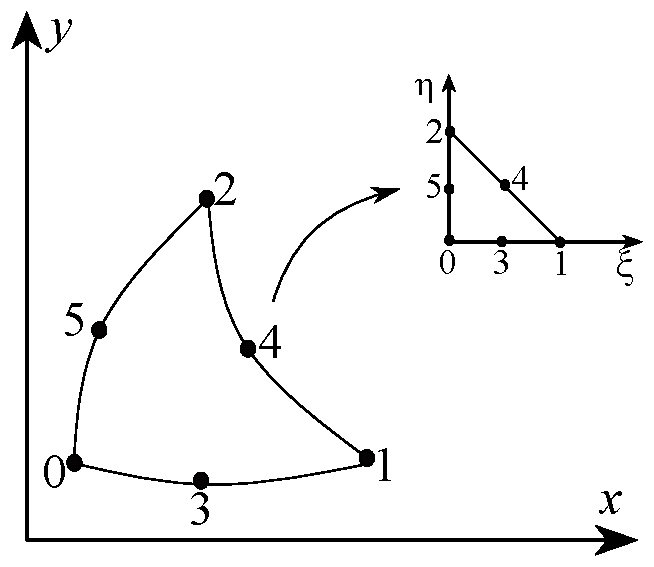
\includegraphics[scale=0.5,trim=0cm 0cm 0cm 0cm, clip=true]{Imagens/Cap2/element2d.pdf}}\\
	\subfloat[Elemento Finito 3d.\label{fig:elementofinito3d}]{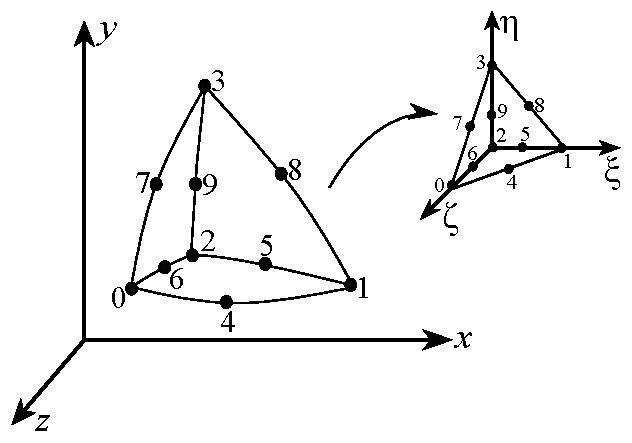
\includegraphics[trim=0 0 0 0,clip,scale=0.65]{Imagens/Cap2/element3d.pdf}}
	\caption{Elementos Finitos: representação espacial e paramétrica}
\end{figure}

\clearpage



\subsection{Implementação Computacional} \label{subsection:DFCComputationalCode}


O Algoritmo que descreve a implementação computacional tanto de problemas utilizando o método dos elementos finitos, quanto para problemas utilizando a análise Isogeométrica, é apresentado no Alg. \ref{alg:fluid_temporalIntegration}.

\begin{algorithm}
	\caption{Algoritmo para problemas de dinâmica dos fluidos computacional}
	\label{alg:fluid_temporalIntegration}
	\begin{algorithmic}[1]
		\For {o passo de tempo $0$ até \timeInterval} 
		\State $i=0$;
		\State Predição da solução: aplicação das Eq. \eqref{eq:Pred1}, Eq. \eqref{eq:Pred2} e Eq. \eqref{eq:Pred3};
		\While{($\epsilon$ < tolerância)}
		\State $i$++;
		\State Interpolação das variáveis do problema: aplicação da Eq. \eqref{eq:approx_accelerationI}, Eq. \eqref {eq:approx_velocityI} e Eq. \eqref{eq:approx_pressI};
		\State Cálculo do incremento nas variáveis do problema: $\Acceleration_{n+1}$ e $\Press_{n+1}$ de acordo com as Eq. \eqref{eq:NR1} e Eq. \eqref{eq:NR2};
		\State Atualização da solução: calculadas de acordo com Eq. \eqref{update1}, Eq. \eqref{update2} e Eq. \eqref{update3}.
		\State Cálculo do erro:
		\begin{align}
		\epsilon =\left\| \NNSM^i \right\|_{L^2}
		\end{align}
		\EndWhile
		\EndFor
	\end{algorithmic}
\end{algorithm}


Escrever sobre c++ e petsc, MUMPS


\section{Verificação e Aplicações}

Para a verificação dos códigos baseados no método dos elementos finitos, adotam-se 2 exemplos muito populares nas bibliografias: Escoamento sobre um cilindro 2D e o problema da cavidade quadrada 3D, os quais são apresentados na subseções sequentes.

\subsection{Escoamento sobre um cilindro - 2D} \label{subsection:escoamentocil2d}

O estudo do problema de um escoamento sobre um cilindro 2D teve como principal intuito a análise dos coeficientes aerodinâmicos medidos ao longo do tempo e verificar consequentemente se o modelo é capaz de reproduzir os fenômenos relacionados à formação e desprendimento de vórtices característicos desse problema. Para isso, diferentes números de Reynolds ($\Reynolds$) foram estudados, $\Reynolds$ = 40, 100 e 1000, os quais são calculados de acordo com a seguinte equação:

\begin{align}
	\Reynolds = \frac{\rho L \lVert\velocinfty\lVert}{\viscosity} = \frac{L \lVert \velocinfty \lVert}{\kviscosity}, \label{eq:Reynolds}
\end{align}

\noindent com $L$ a dimensão característica do problema, sendo nesse caso o diâmetro do cilindro, e $\kviscosity$ a viscosidade cinemática do fluido. 

\begin{figure}[!htb]
	\centering
	\subfloat[Geometria e condições de contorno.\label{fig:cilindro2d_geometria}]{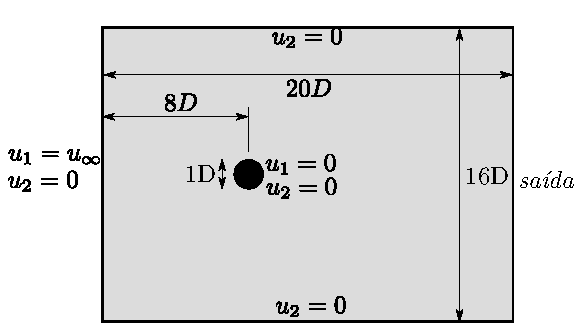
\includegraphics[scale=1.0,trim=0cm 0cm 0cm 0cm, clip=true]{Imagens/Cap2/cilindro2d.pdf}}\\
	\subfloat[Discretização espacial.\label{fig:cilindro2d_malha}]{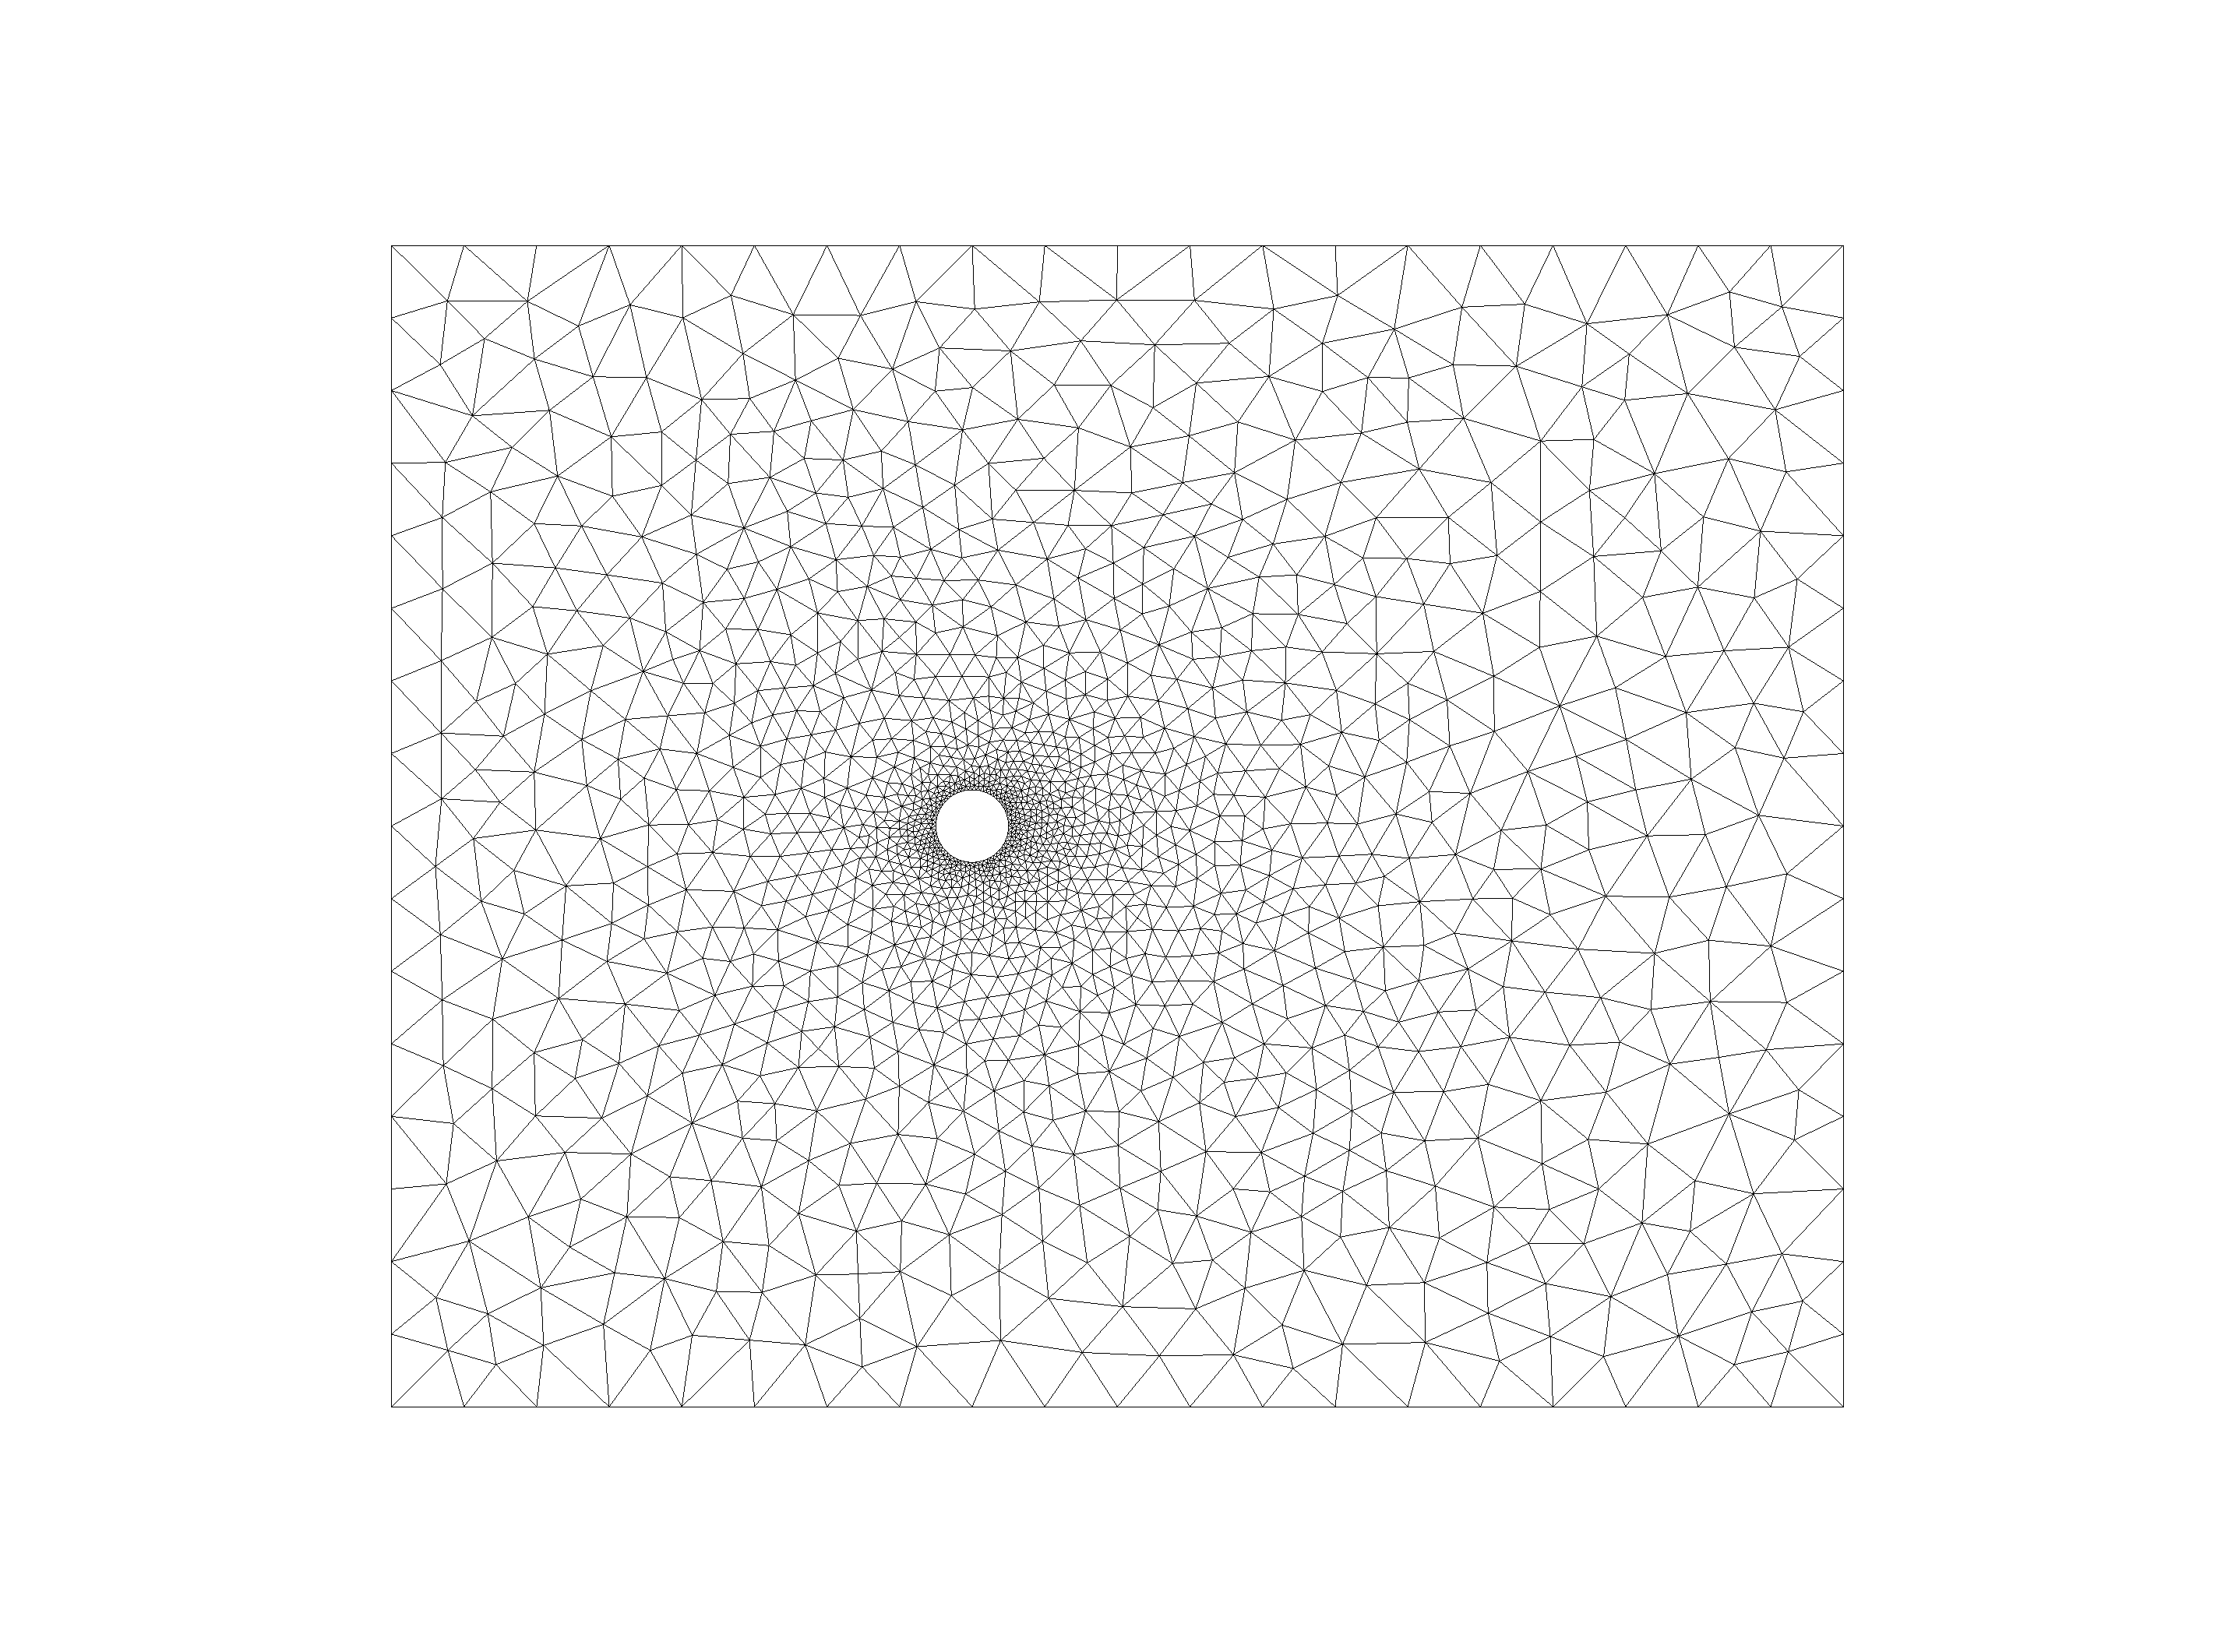
\includegraphics[trim=170 120 170 130,clip,scale=0.2]{Imagens/Cap2/MeshCylinder2D.eps}}
	\caption{Cilindro 2D: Geometria, condições de contorno e malha de elementos finitos.}
\end{figure}


A geometria e condições de contorno são apresentadas na Fig. \ref{fig:cilindro2d_geometria}. Como pode-se observar trata-se de um domínio retangular, parametrizado em função do diâmetro do cilindro, com um perfil constante de velocidade na entrada e condição de parede lisa nas paredes superior e inferior (velocidade normal à parede $u_{n}$ = 0). No contorno denominado como \textit{saída}, não se conhece o comportamento do escoamento, desta forma, determina-se sua posição no domínio computacional a uma distância grande o suficiente de maneira a não interferir no comportamento do escoamento. Além disso, prescreve-se uma condição de contorno dita artificial, que consiste em $\stresstensor \normal = \mathbf{0}$.

Na Fig. \ref{fig:cilindro2d_malha} pode-se observar a malha não-estruturada de elementos finitos utilizada para esse problema, composta por 3122 elementos triangulares quadráticos e 6376 nós. O problema foi simulado para um velocidade de entrada $u_{\infty} = 1,0$, $\rho = 1,0$, $\timeStep = 0,05$, e $\specRadius = 0,5$. 

Para o cálculo dos coeficientes aerodinâmicos é necessário definir-se primeiramente as forças de arrasto - horizontal ($F_D$) e de sustentação - vertical ($F_L$), que são induzidas por tensões desviadores e hidrostáticas e são calculadas pelas seguintes equações:

\begin{align}
F_D = \int_{\boundary_{c}} \stresstensor_{1j}n_{j} d\boundary_{c},
\end{align}

\begin{align}
F_L = \int_{\boundary_{c}} \stresstensor_{2j}n_{j} d\boundary_{c},
\end{align}

\noindent nas quais o símbolo $\boundary_{c}$ representa o contorno do cilindro e $n$ é o vetor normal à essa superfície. Os coeficientes de arrasto e sustentação são definidos respectivamente por:

\begin{align}
	C_D = \frac{F_D}{0,5\rho \lVert \velocity \lVert^{2} L},
\end{align}

\begin{align}
	C_L = \frac{F_L}{0,5\rho \lVert \velocity \lVert^{2} L},
\end{align}.

Devido ao fenômeno de desprendimento de vórtices que ocorre a partir de determinado número de Reynolds do escoamento, é usual determinar-se a frequência deste fenômeno através do número adimensional de Strouhal ($\Strouhal$), dado por:

\begin{align}
	\Strouhal = \frac{f_{V}L}{\lVert \velocity \lVert},
\end{align}.

\noindent com $f_{V}$ sendo a frequência de desprendimento dos vórtices.

Como pode-se observar na Fig. \ref{fig:cilindro_coeficientes} para $\Reynolds = 40$, os coeficientes de arrasto e de sustentação, após o escoamento entrar em fase estacionária, se mantém constantes ao longo de todo o tempo de análise. Isso ocorre, visto que para Reynolds entre 5 à 50, aproximadamente, formam-se dois vórtices simétricos e estacionários na região logo após o cilindro. Posteriormente, o par de vórtices se quebra e passa existir a chamada esteira de Von Karmán, que ocorre devido à formação de vórtices de maneira alternada entre as regiões superior e inferior do cilindro, o que pode ser notado também na Fig. \ref{fig:cilindro_coeficientes}  para $Re = 100$ e $Re=1000$. Os valores do coeficiente de Strouhal, para $Re = 100$ e $Re=1000$, foram de 0,1716 e 0,2454 respectivamente. Os valores obtidos para os coeficientes aerodinâmicos foram os esperados para o problema em questão (ver, por exemplo, \citeonline{Tonon:2016,Henderson:1997}).

\begin{figure}[!htb]
	\centering
	\subfloat[\label{fig:cilindro_Cd}Coeficiente de arrasto $ C_D$.]{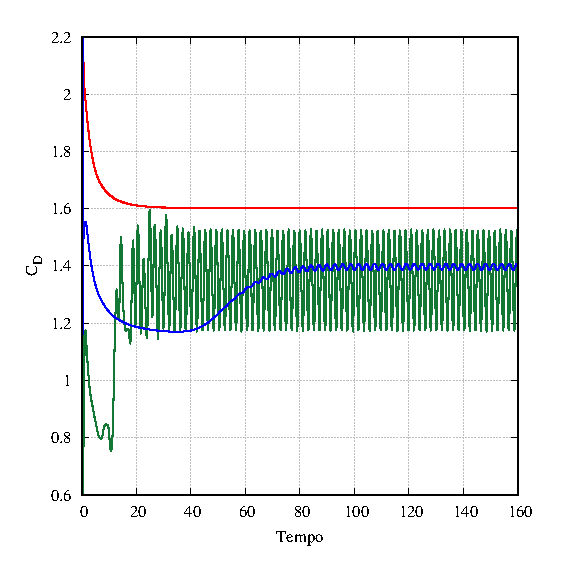
\includegraphics[scale=1,trim=0cm 0cm 0cm 0cm, clip=true]{Imagens/Cap2/DragRe.eps}}\\ 
	\subfloat[\label{fig:cilindro_Cl}Coeficiente de sustentação $C_L$.]{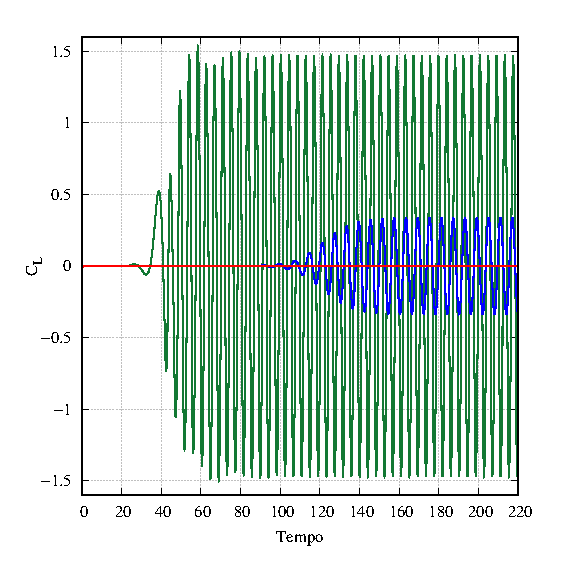
\includegraphics[scale=1,trim=0cm 0cm 0cm 0cm, clip=true]{Imagens/Cap2/LiftRe.eps}}\\ 
	{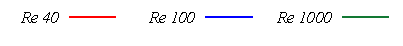
\includegraphics[scale=1.3]{Imagens/Cap2/Legenda.pdf}}
	\caption{Cilindro 2D: Coeficientes aerodinâmicos. }
	\label{fig:cilindro_coeficientes}
\end{figure}

Nas Fig. \ref{fig:cilindro_2d_pressao} e Fig. \ref{fig:cilindro_2d_velocidade} podem ser observados os campos de pressão e velocidade em um tempo $t=11,5$ da análise para $Re = 100$. Pode-se notar nessas imagens, a formação e os desprendimentos de vórtices na esteira de Von Karmán, característico do escoamento para o número de Reynolds simulado.

\begin{figure}[!htb]
	\centering
	\subfloat[\label{fig:cilindro_2d_pressao}Campo de pressão]{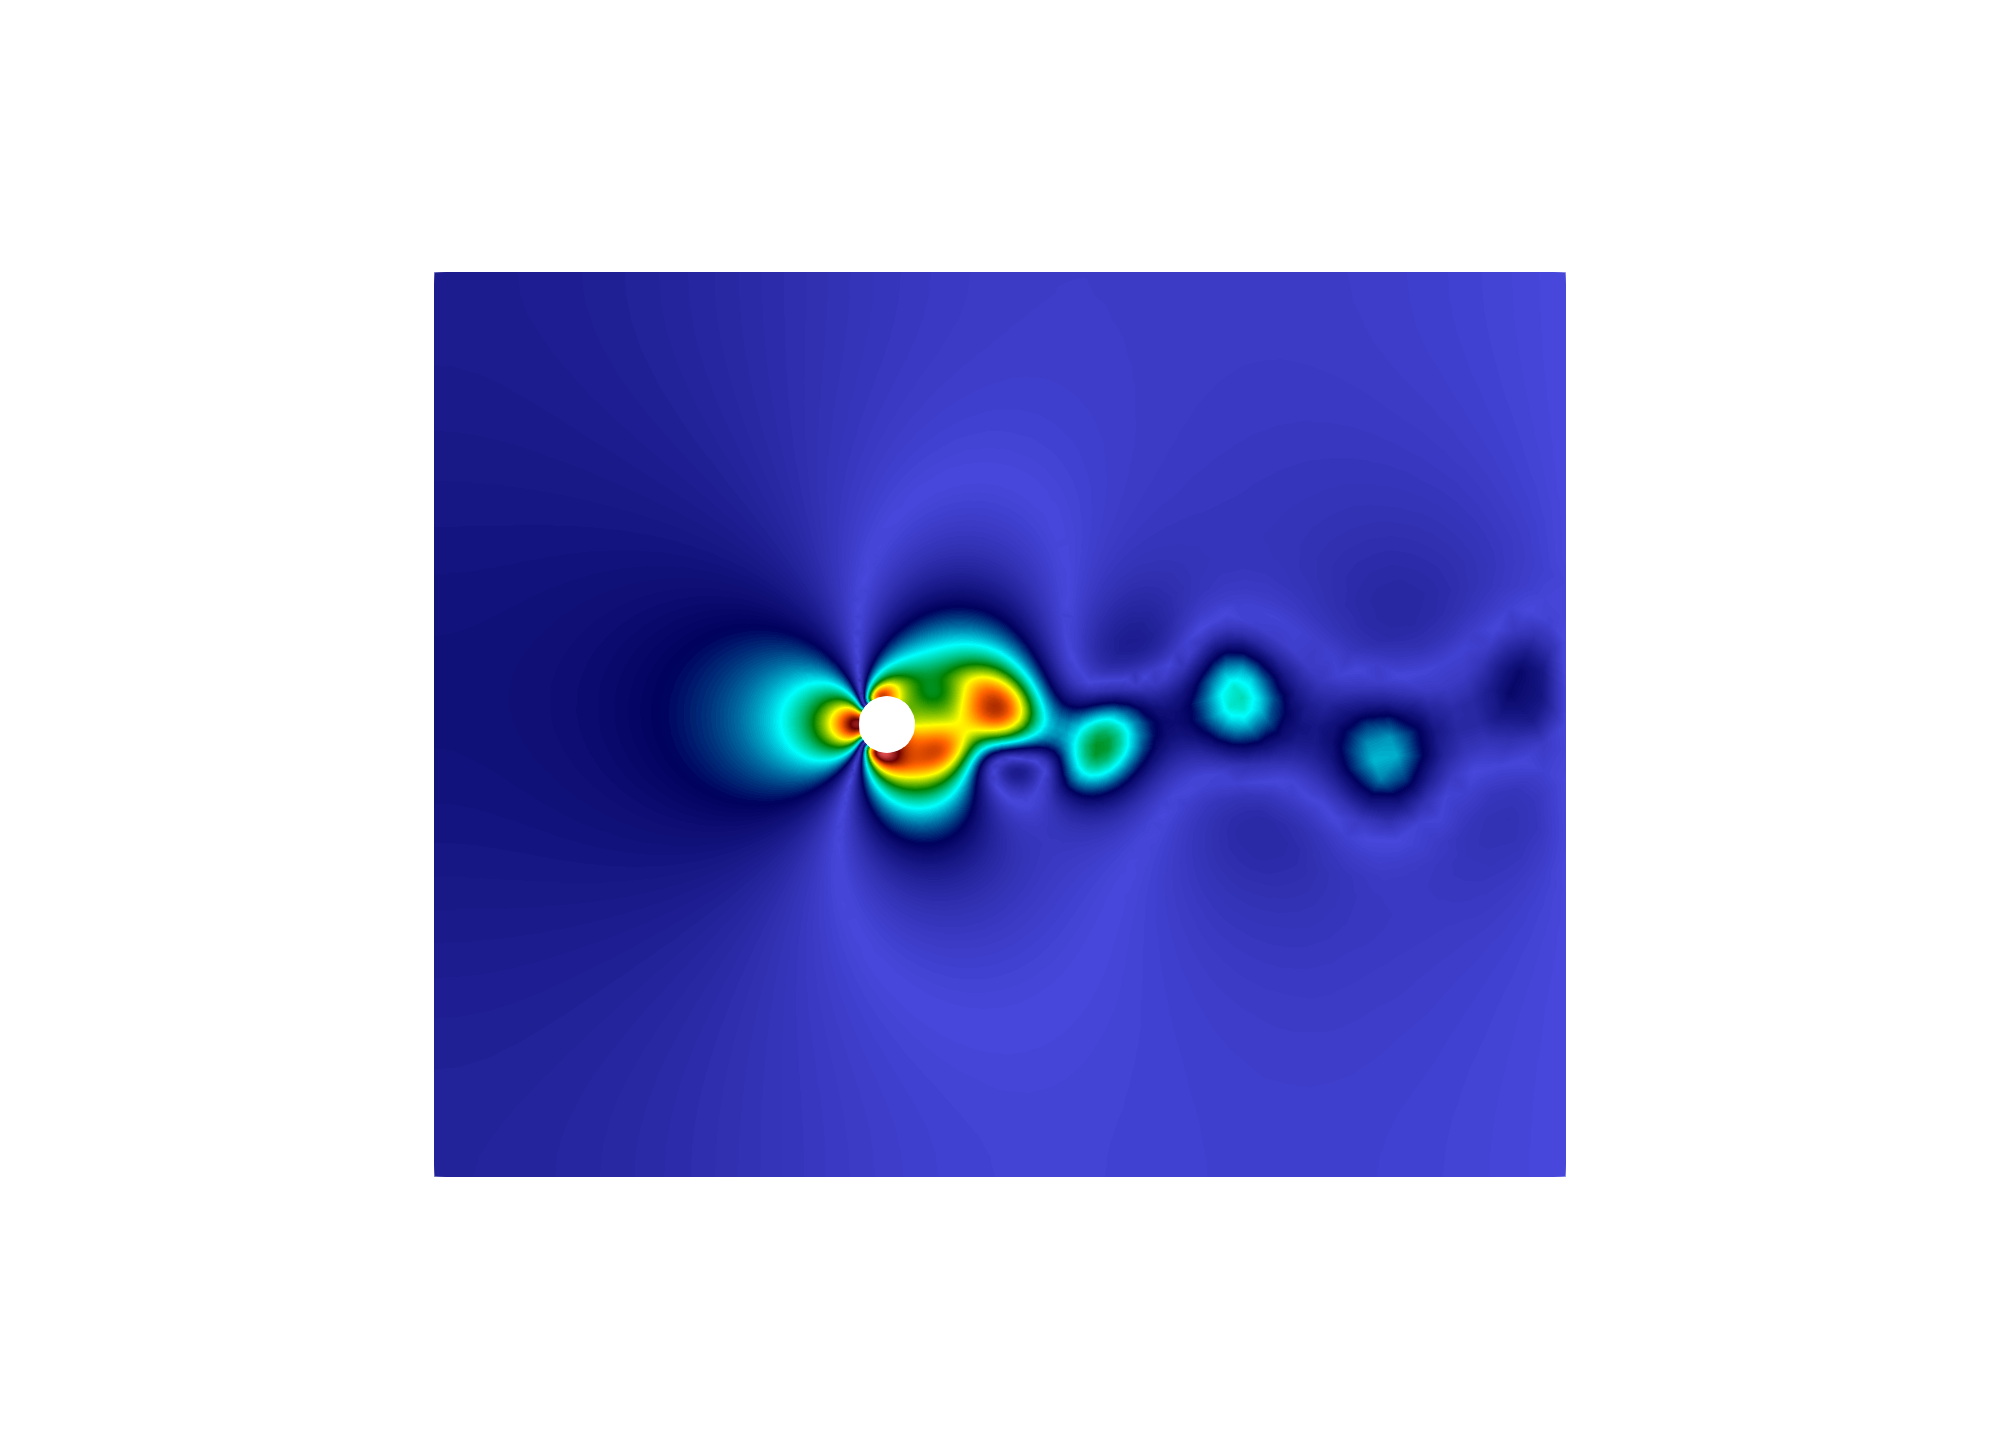
\includegraphics[scale=0.2,trim=15cm 9cm 14cm 9cm, clip=true]{Imagens/Cap2/pressaoRe100.png}}\\ 
	\subfloat[\label{fig:cilindro_2d_velocidade}Campo de velocidade]{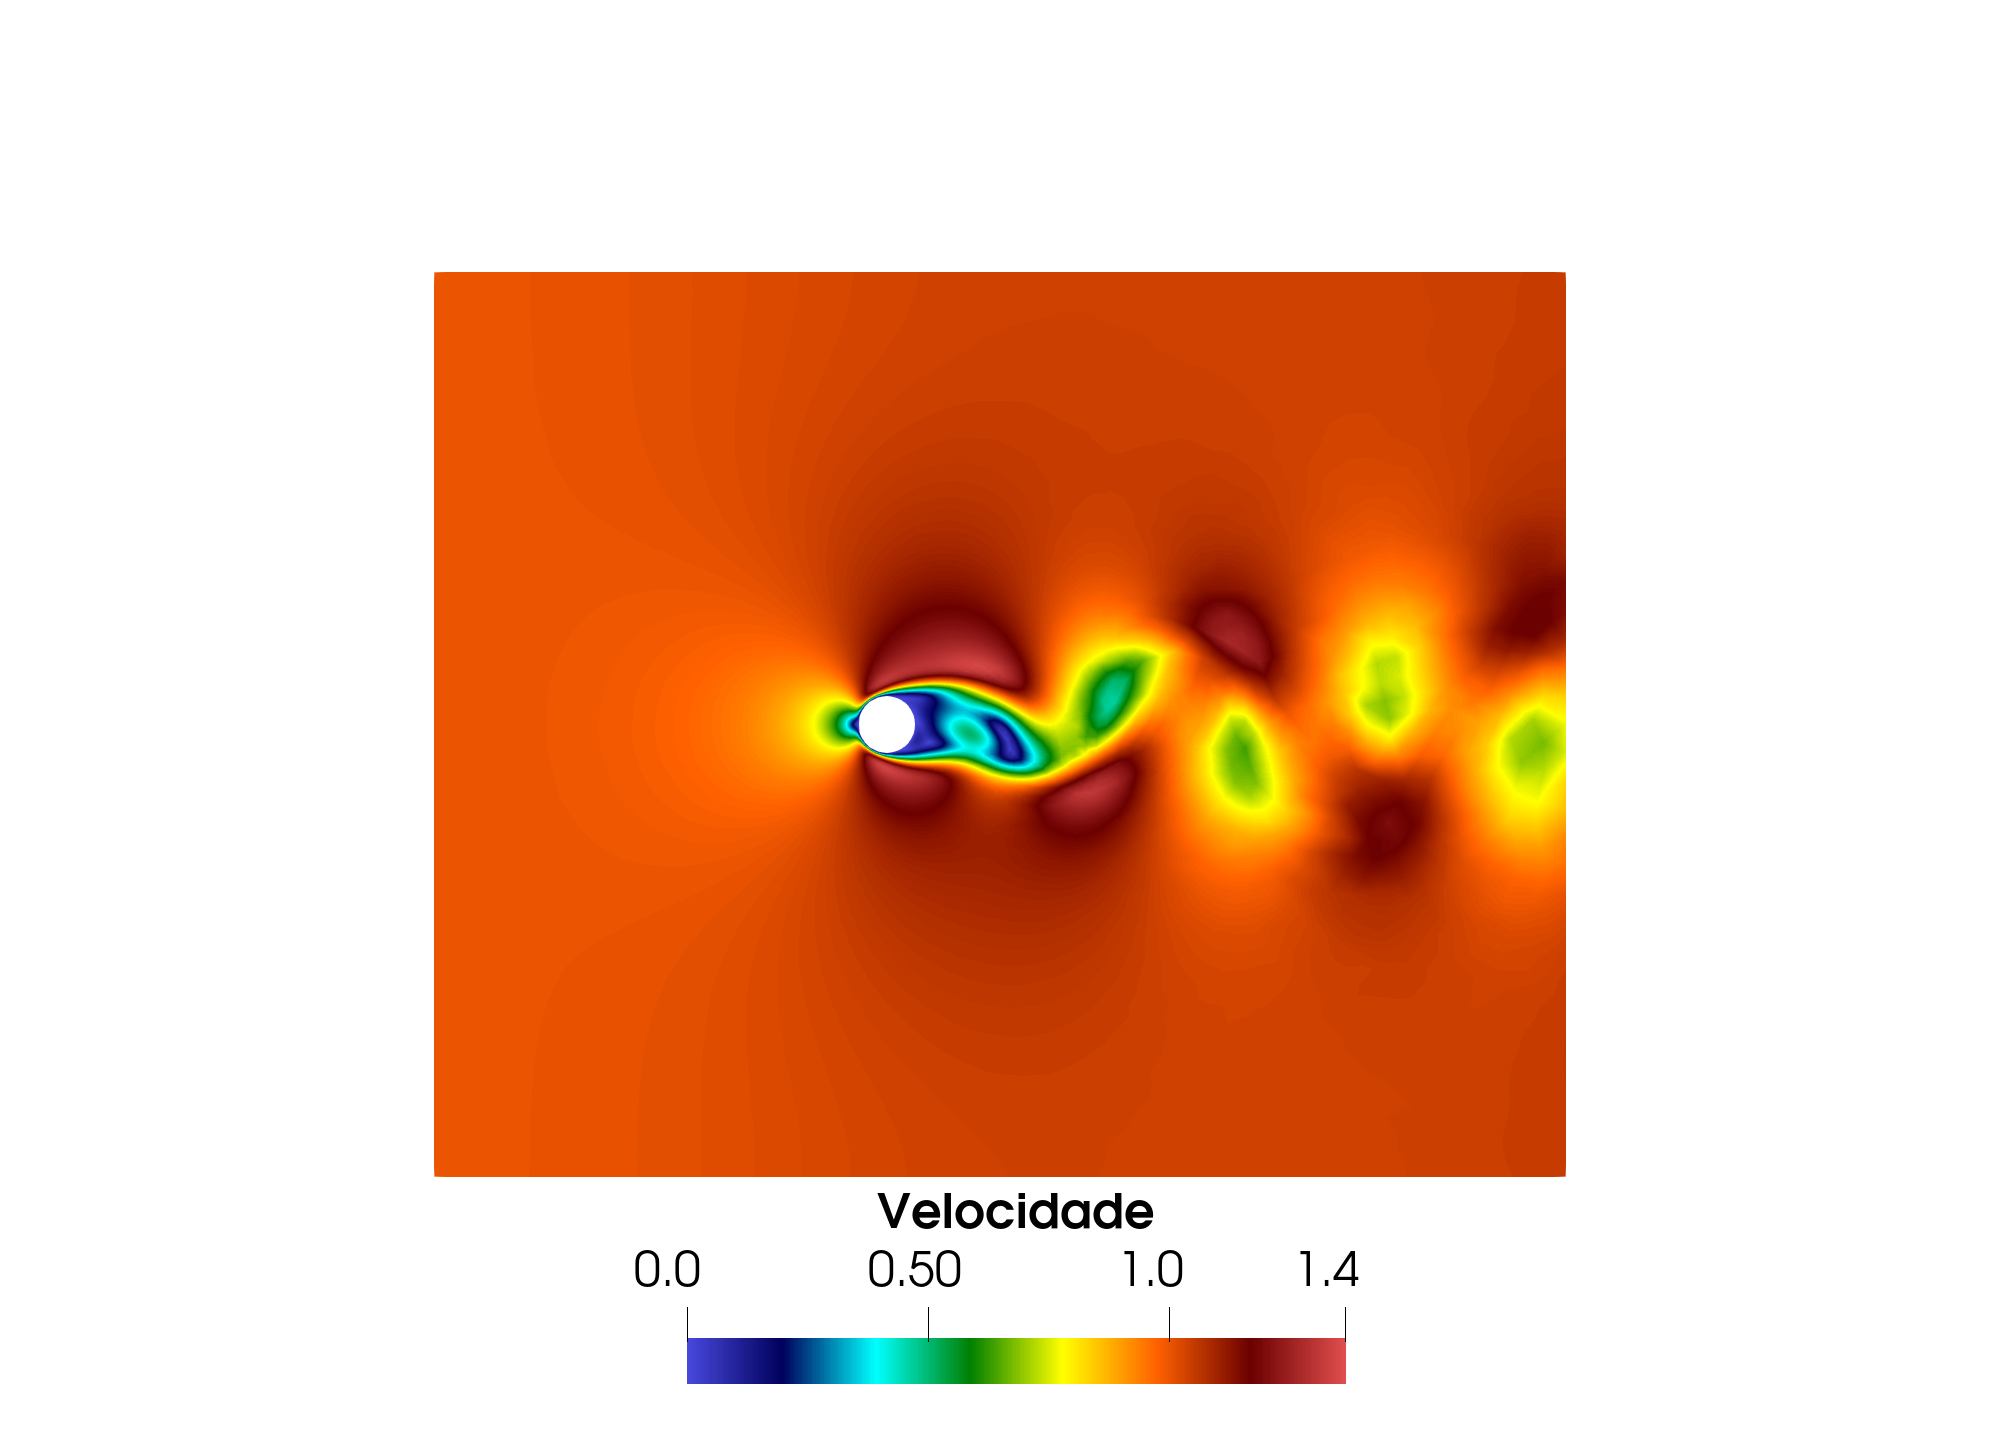
\includegraphics[scale=0.2,trim=15cm 1cm 14cm 9cm, clip=true]{Imagens/Cap2/velocitymagnitude.png}}
	\caption{Cilindro 2D: Campos de pressão e de velocidade para um escoamento com $Re = 100$ }
	\label{fig:cilindro_campos}
\end{figure}


\subsection{Cavidade Quadrada - 3D} \label{subsec:CavQua3d}

Para a verificação do código 3D utilizando elementos finitos o problema de uma cavidade quadrada com velocidade prescrita $u_{\infty}$ em sua parede superior foi estudado. A geometria do problema em questão e o conjunto de suas condições de contorno são apresentadas na Fig. \ref{fig:cavidade_geometria}. As paredes da cavidade são rígidas, com paredes laterais e do fundo com condição de aderência, e adicionalmente, velocidade $u_{z}=0$, condição de parede lisa, nas paredes das faces frontal e posterior. A cavidade possui na direção $z$ uma espessura de 0,03. A discretização espacial em elementos finitos utilizada é apresentada na Fig.  \ref{fig:cavidade_malha}, a qual consiste em 7252 elementos tetraédricos quadráticos e 14727 nós.

O problema é estudado para os números de Reynolds: 100, 400 e 1000. O número de Reynolds foi calculado de acordo com Eq. \eqref{eq:Reynolds}, com $L$ equivalente ao comprimento do lado da cavidade. O problema foi simulado para uma velocidade na parede superior de $\velocity_{\infty} = 1,0$, $\rho = 1,0$, $\timeStep = 0,05$, e $\specRadius = 0$, sendo a viscosidade do fluido variada de modo a alterar o número de Reynolds. A simulação foi mantida até que se atingiu o estado estacionário de escoamento. 

\begin{figure}[!htb]
	\centering
	\subfloat[Geometria e condições de contorno.\label{fig:cavidade_geometria}]{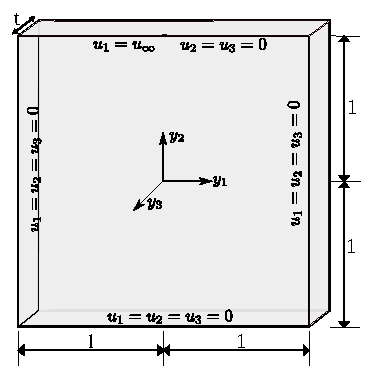
\includegraphics[scale=1.0,trim=0cm 0cm 0cm 0cm, clip=true]{Imagens/Cap2/cavidade.pdf}} \quad
	\subfloat[Discretização espacial.\label{fig:cavidade_malha}]{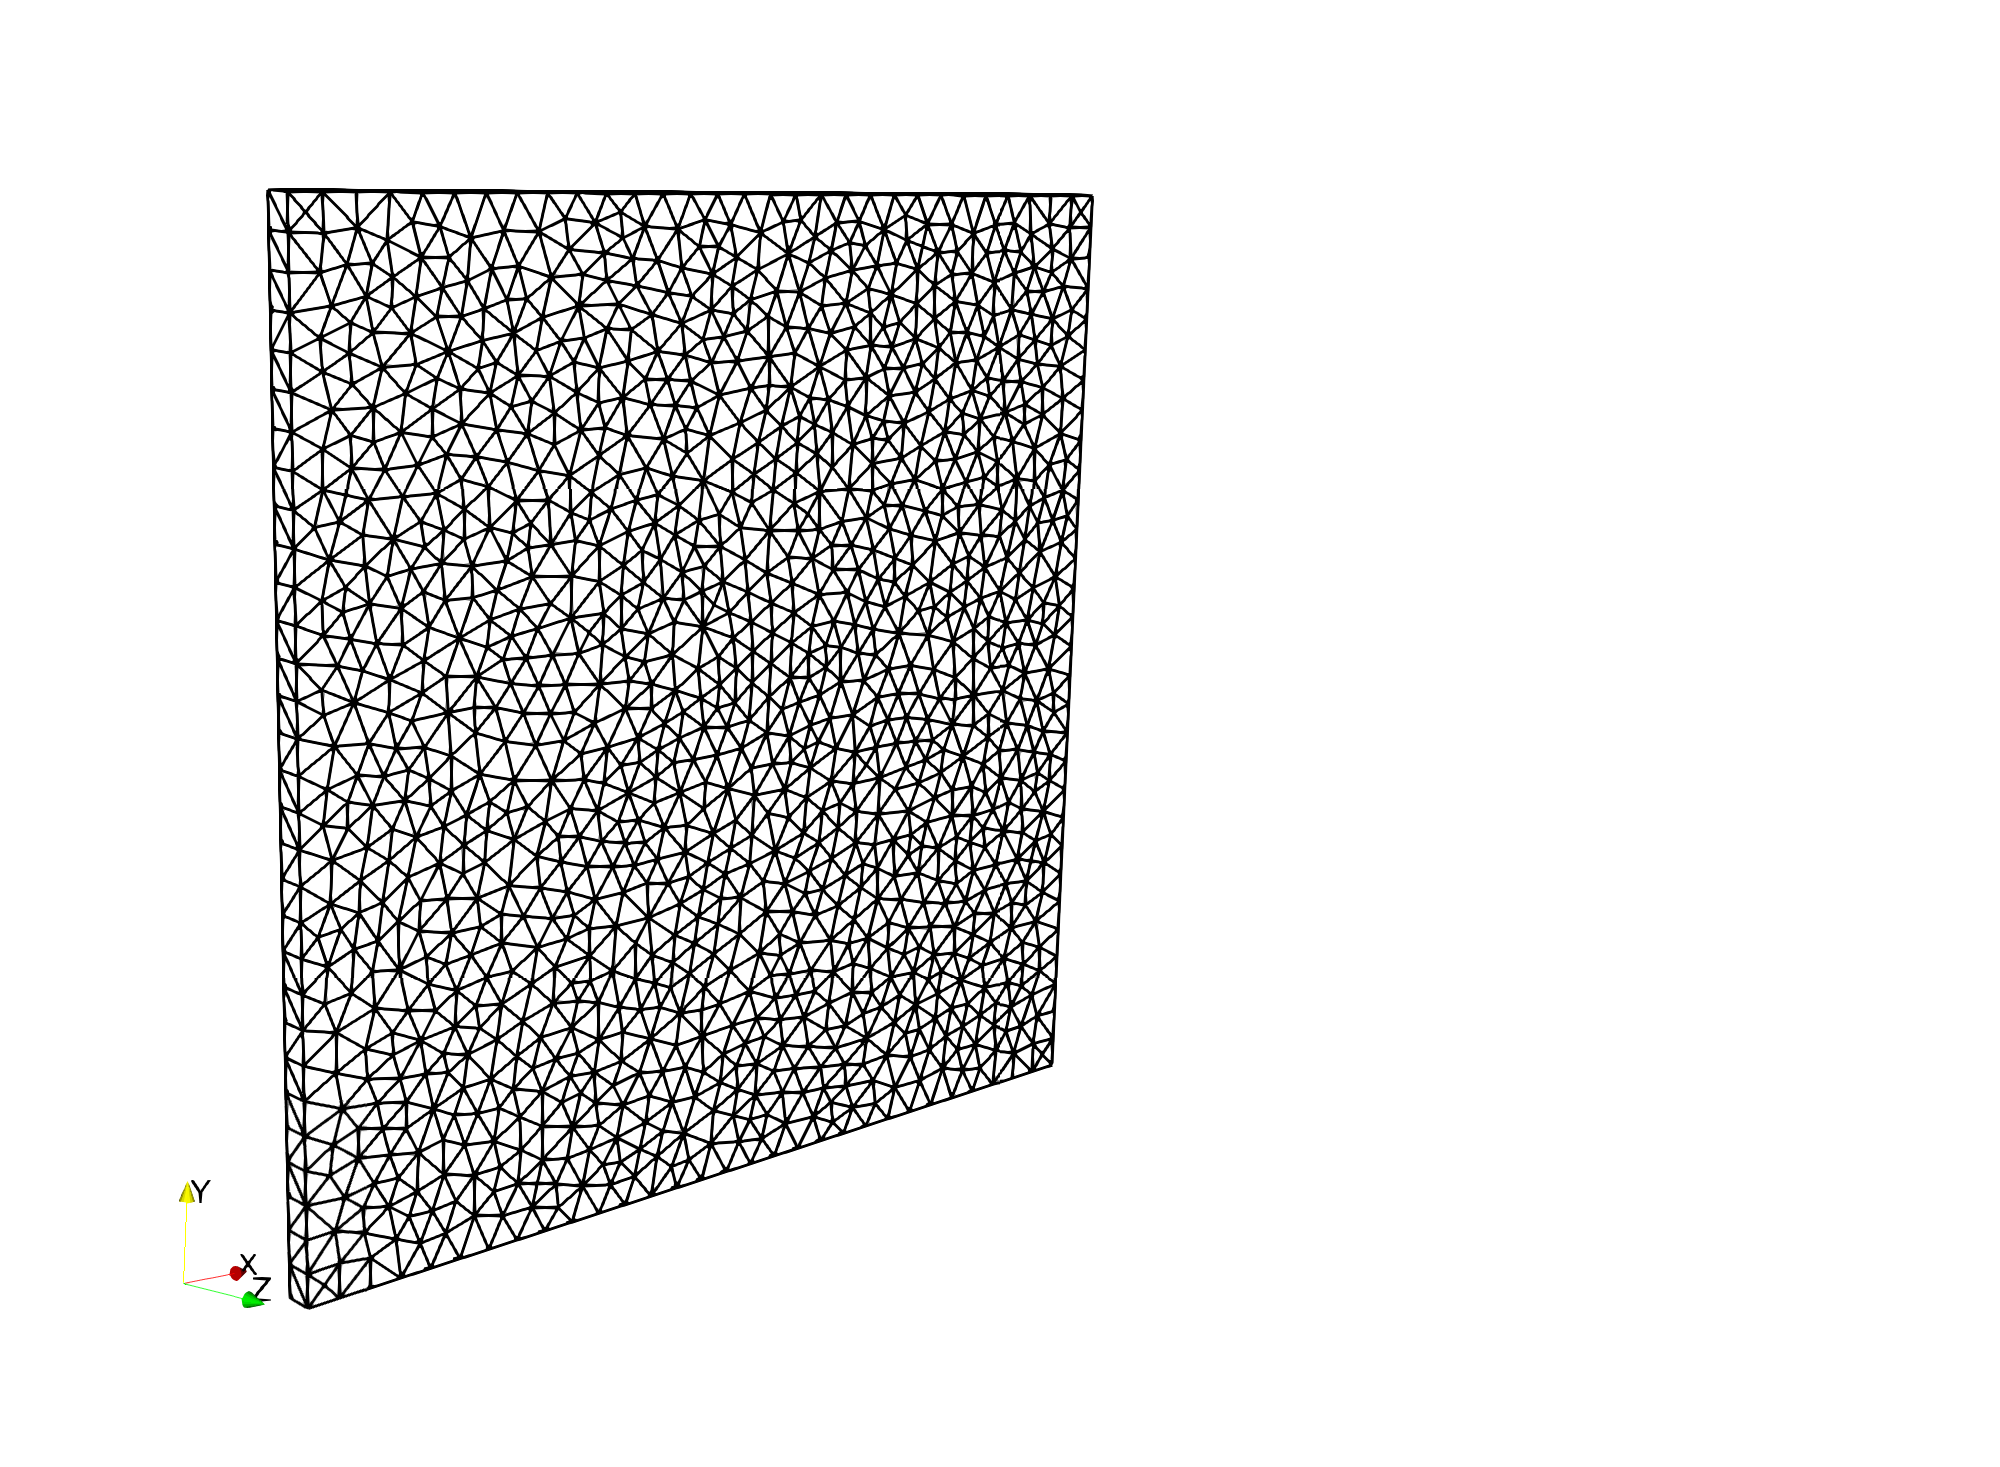
\includegraphics[trim=170 120 850 130,clip,scale=0.15]{Imagens/Cap2/cavitymesh.png}}
	\caption{Cavidade quadrada: Geometria, condições de contorno e malha de elementos finitos.}
\end{figure}

Os perfis de velocidade adimensionalizados ($\velocity/\velocinfty$) horizontal e vertical ao longo de duas linhas centrais nas direções $x$ e $y$ posicionadas no centro da espessura na direção $z$ da cavidade são apresentados na Fig. \ref{fig:cavidade_graficos} e comparados com a referência de \citeonline{GhiaGS:1982}.


\begin{figure}[!t]
	\centering
	\subfloat[\label{fig:cavidade_g_Re100}$Re$=100.]{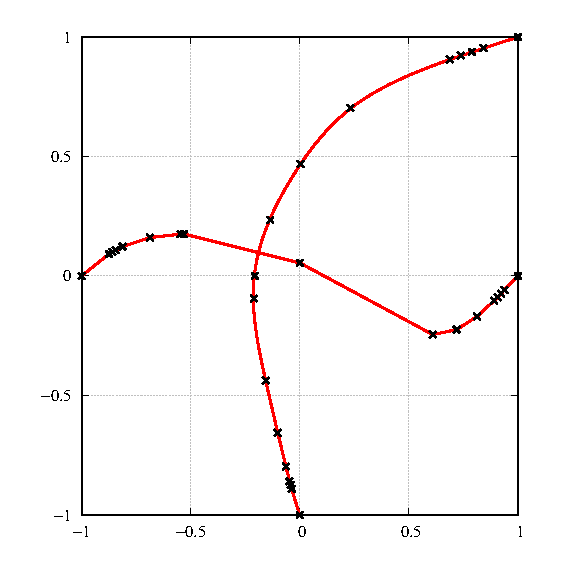
\includegraphics[scale=.8,trim=0.55cm 0.5cm 0.3cm 0.2cm, clip=true]{Imagens/Cap2/cavidade_Re100.eps}} \subfloat[\label{fig:cavidade_g_Re400}$Re$=400.]{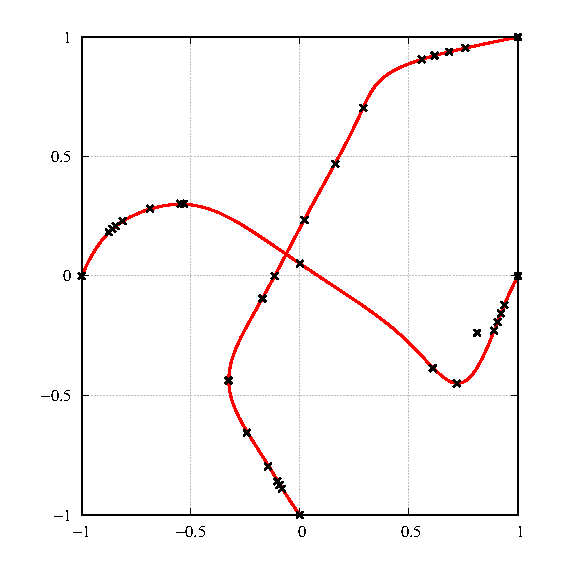
\includegraphics[scale=.8,trim=0.55cm 0.5cm 0.3cm 0.2cm, clip=true]{Imagens/Cap2/cavidade_Re400.eps}}\\ 
	\subfloat[\label{fig:cavidade_g_Re1000}$Re$=1000.]{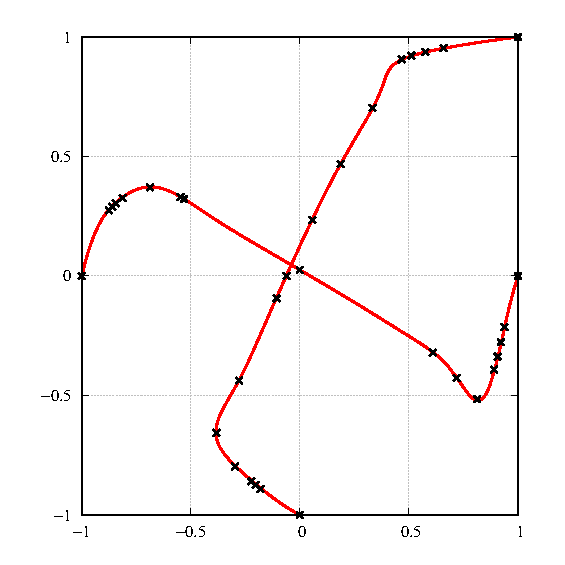
\includegraphics[scale=.8,trim=0.55cm 0.5cm 0.3cm 0.2cm, clip=true]{Imagens/Cap2/cavidade_Re1000.eps}} \\
	\subfloat{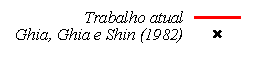
\includegraphics[scale=1.]{Imagens/Cap2/legenda.pdf}} 
	\caption{Cavidade quadrada: Perfis de velocidade adimensionalizados nas direções $x$ e $y$ . }
	\label{fig:cavidade_graficos}
\end{figure}

Os campos de velocidade e de pressão são apresentados nas figuras Fig \ref{fig:cav3d-vel} e \ref{fig:cav3d-press} respectivamente. Ressalta-se que para a solução do problema, por se tratar de um problema com todos os contornos com condição de Dirichlet impostos, a pressão torna-se indefinida. Por esse motivo, prescreveu-se uma pressão $\press = \press_{ref} =  0$ no canto superior direito da cavidade. 


\begin{figure}[!t]
	\centering
	\setlength{\lineskip}{-10pt}
	\subfloat[\label{fig:cavidade_Vel_Re100}$Re$=100.]{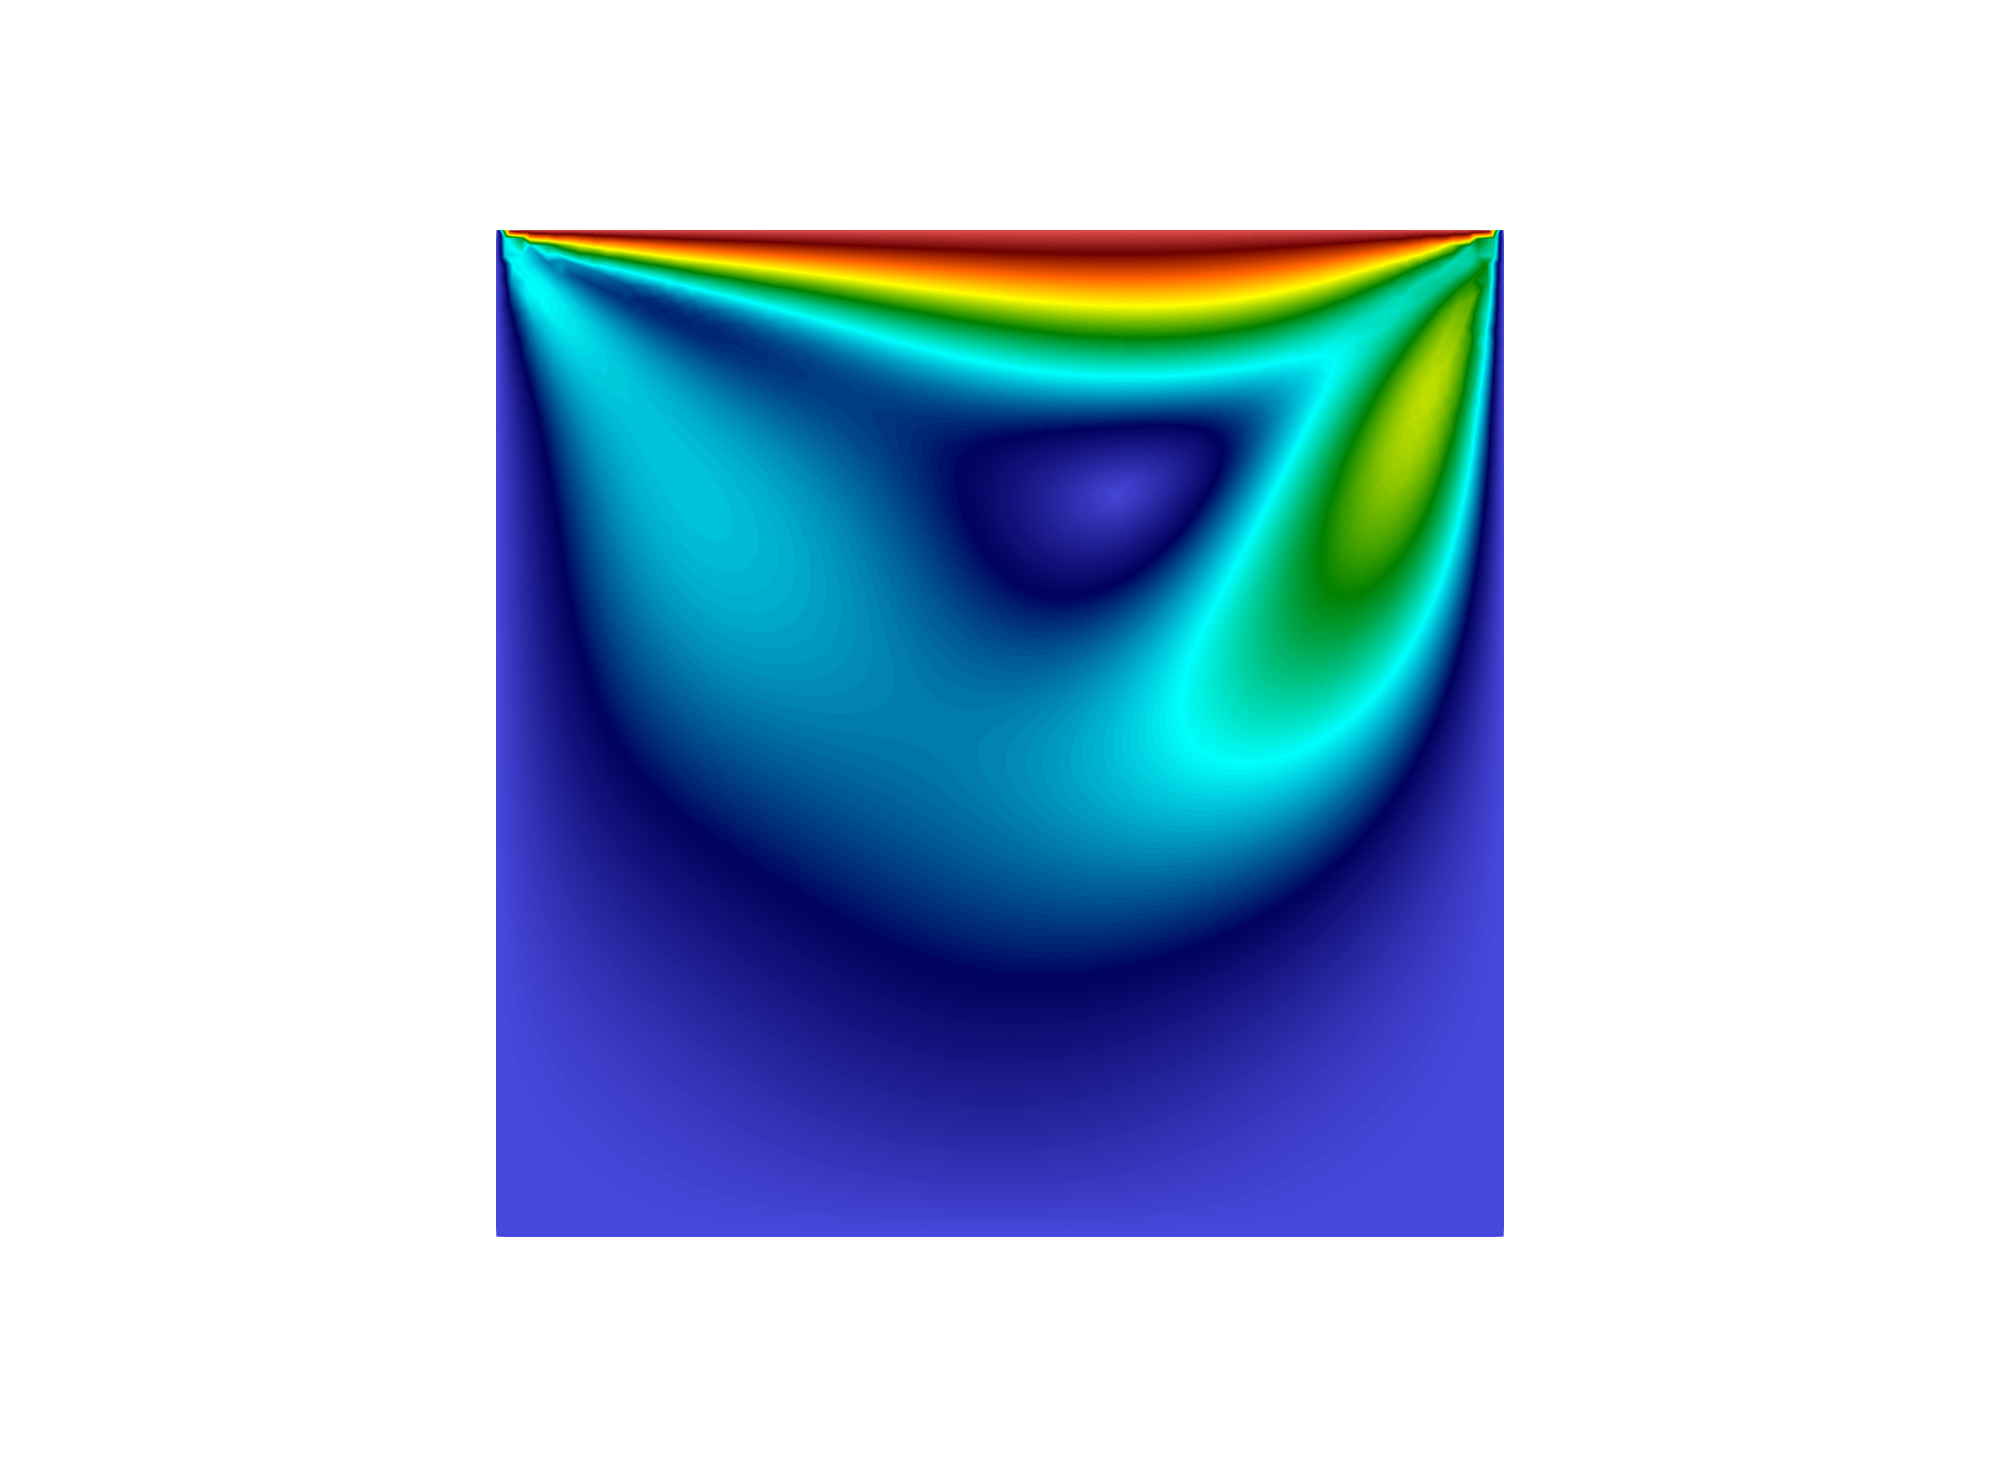
\includegraphics[scale=0.15,trim=15cm 7cm 15cm 7cm, clip=true]{Imagens/Cap2/velocity-Re100.png}} \subfloat[\label{fig:cavidade_Vel_Re400}$Re$=400.]{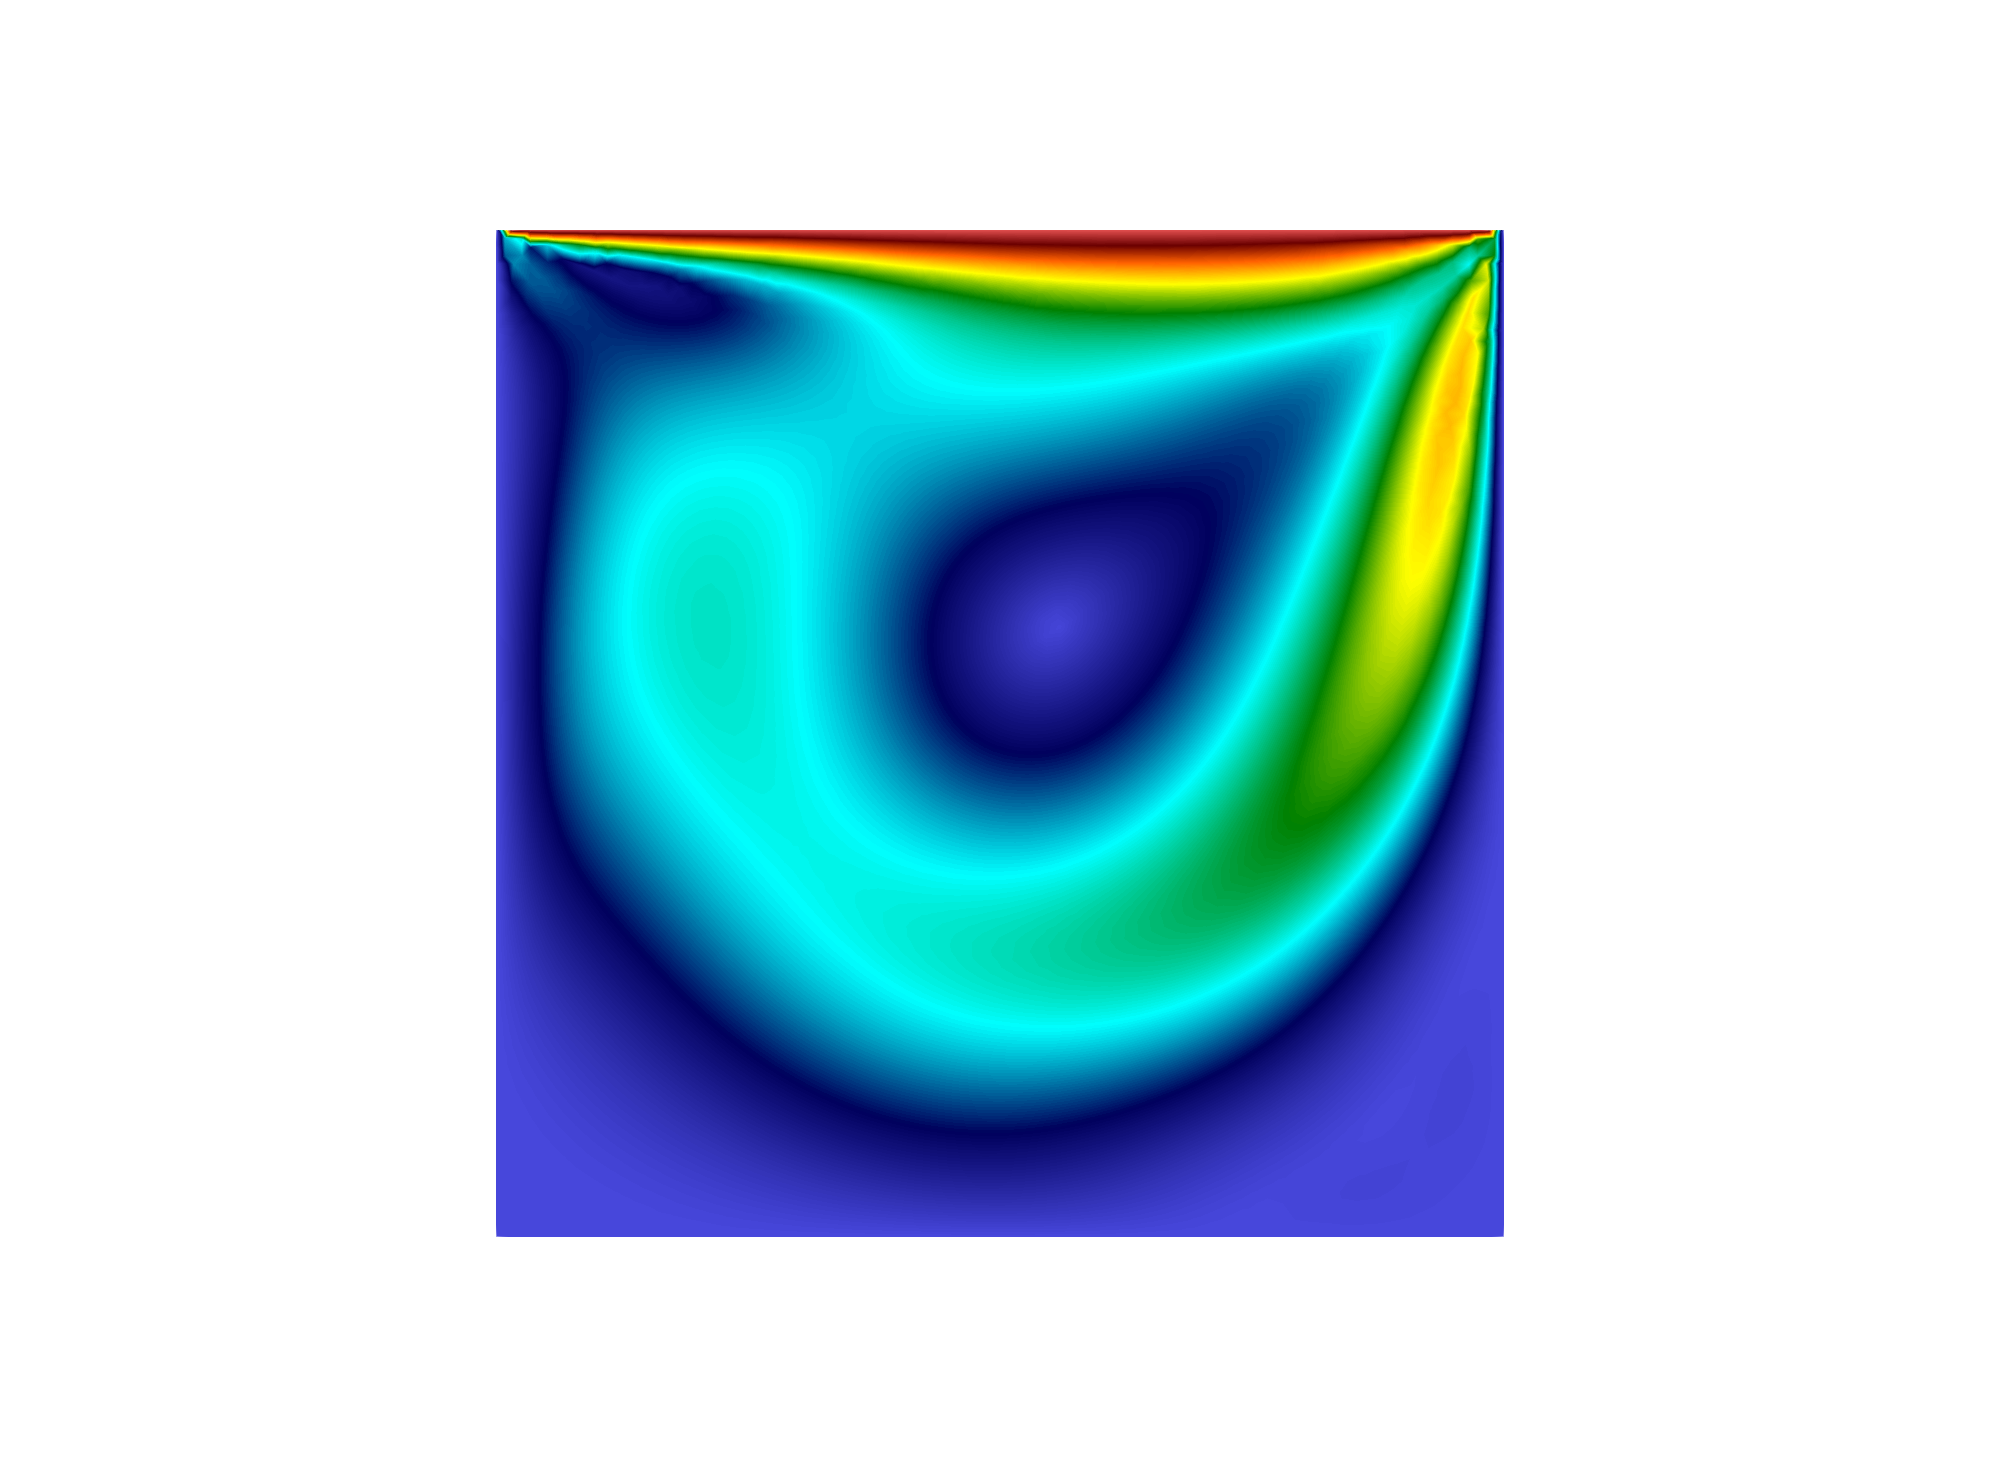
\includegraphics[scale=0.15,trim=15cm 7cm 15cm 7cm, clip=true]{Imagens/Cap2/velocity-Re400.png}}\\ 
	\subfloat[\label{fig:cavidade_Vel_Re1000}$Re$=1000.]{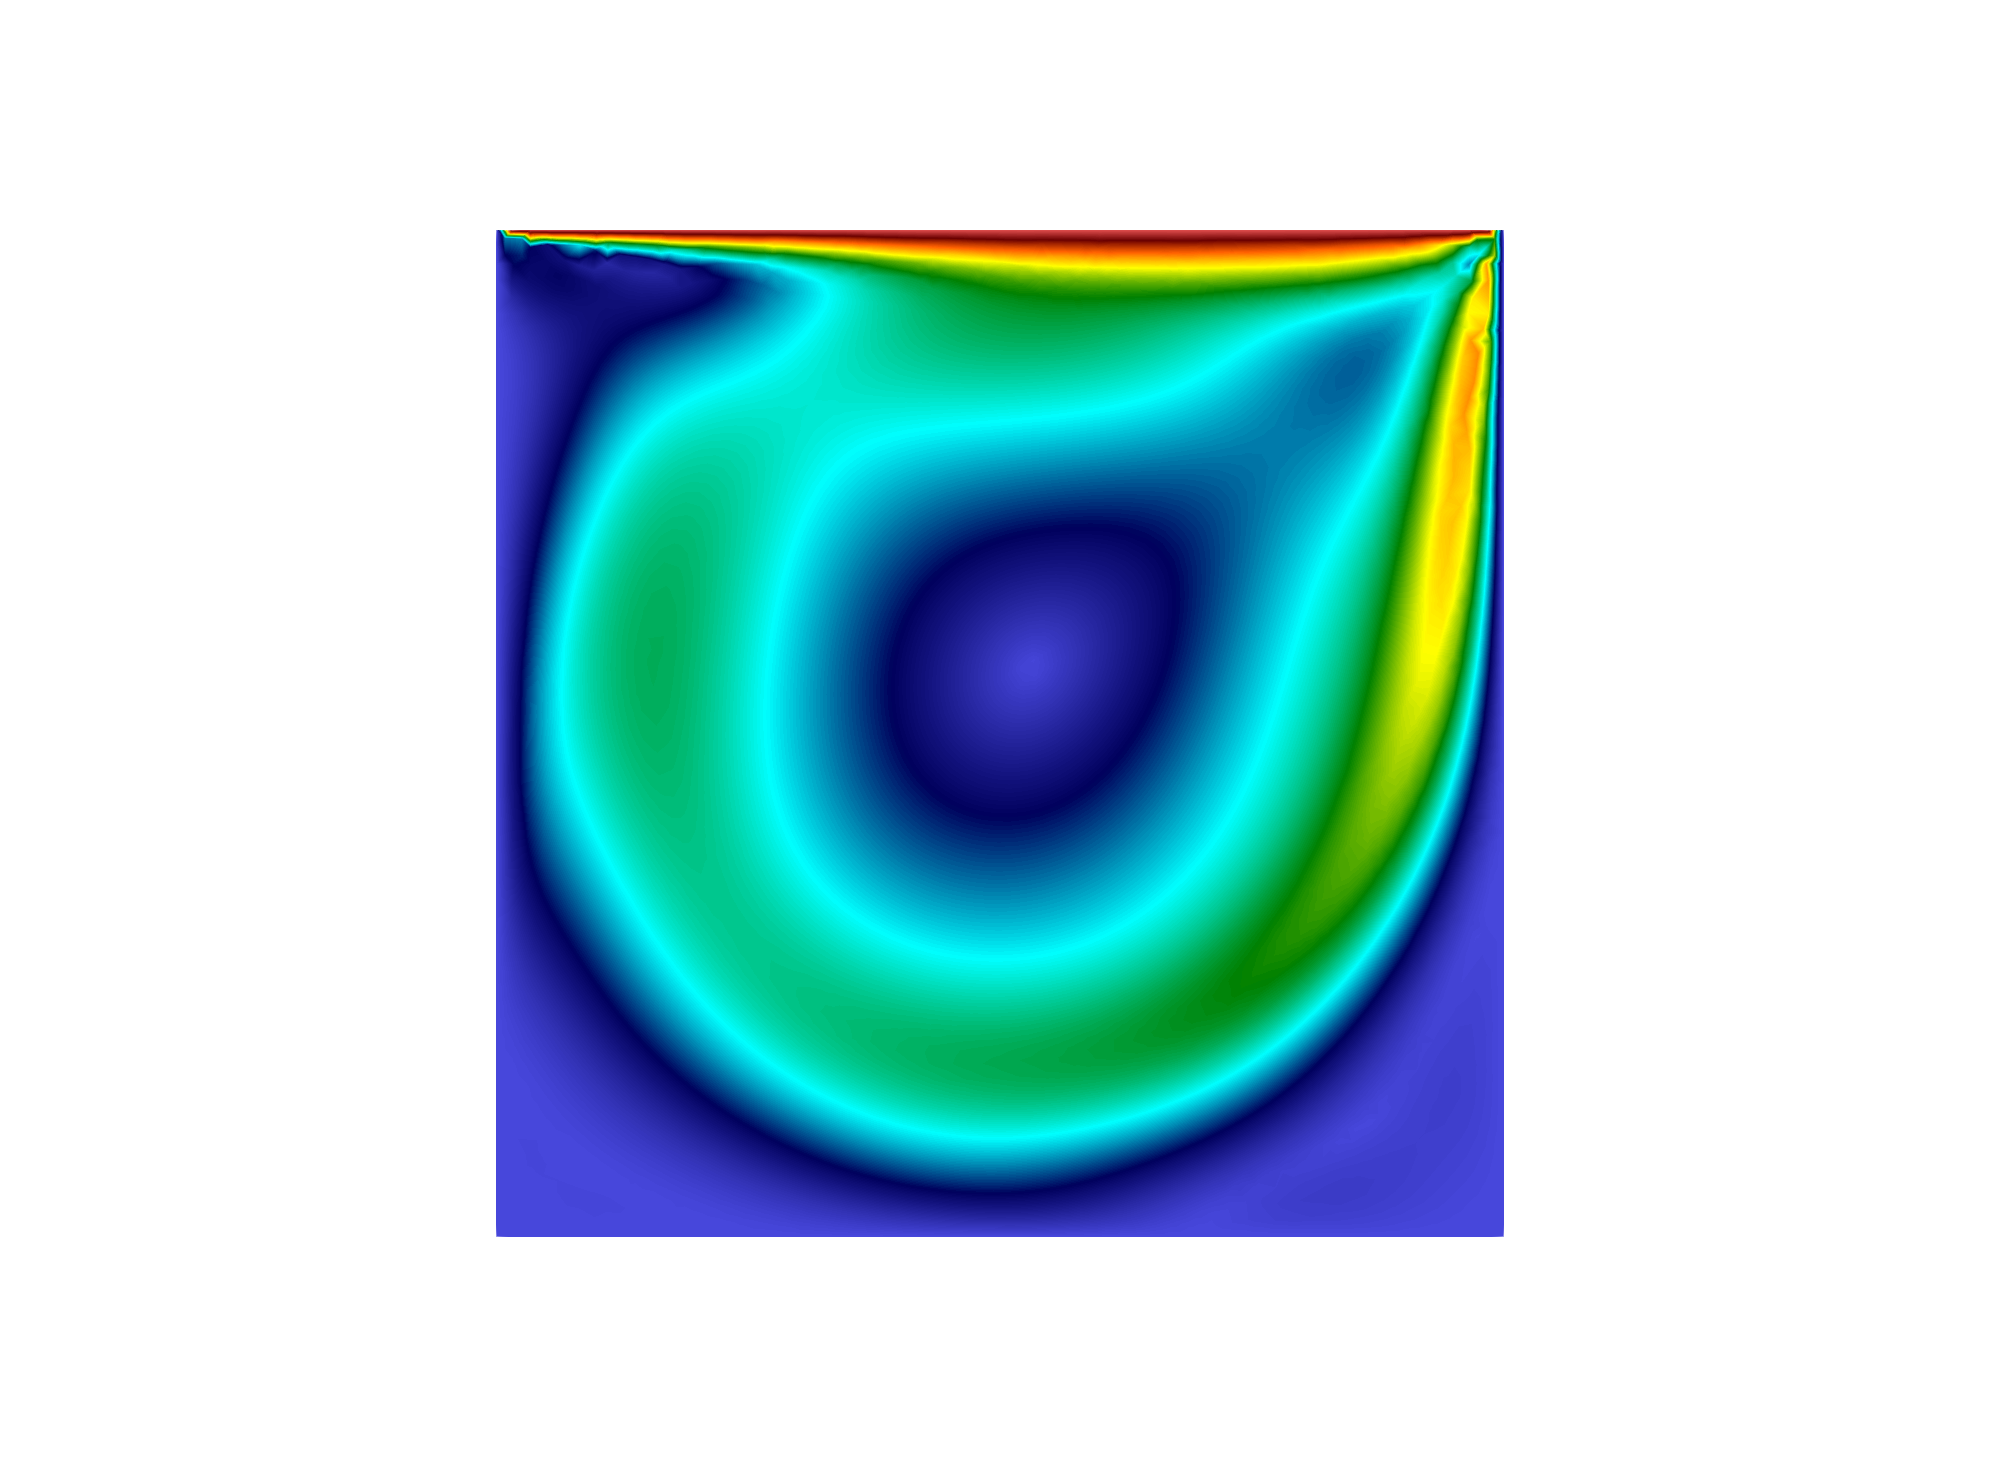
\includegraphics[scale=0.15,trim=15cm 7cm 15cm 7cm, clip=true]{Imagens/Cap2/velocity-Re1000.png}} \\
	%	\subfloat[\label{fig:cavidade_g_Re10000}$Re$=10000.]{\includegraphics[scale=1.1,trim=0.55cm 0.5cm 0.3cm 0.2cm, clip=true]{Imagens/Cap2/cavidade_Re10000.eps}}\\
	\subfloat{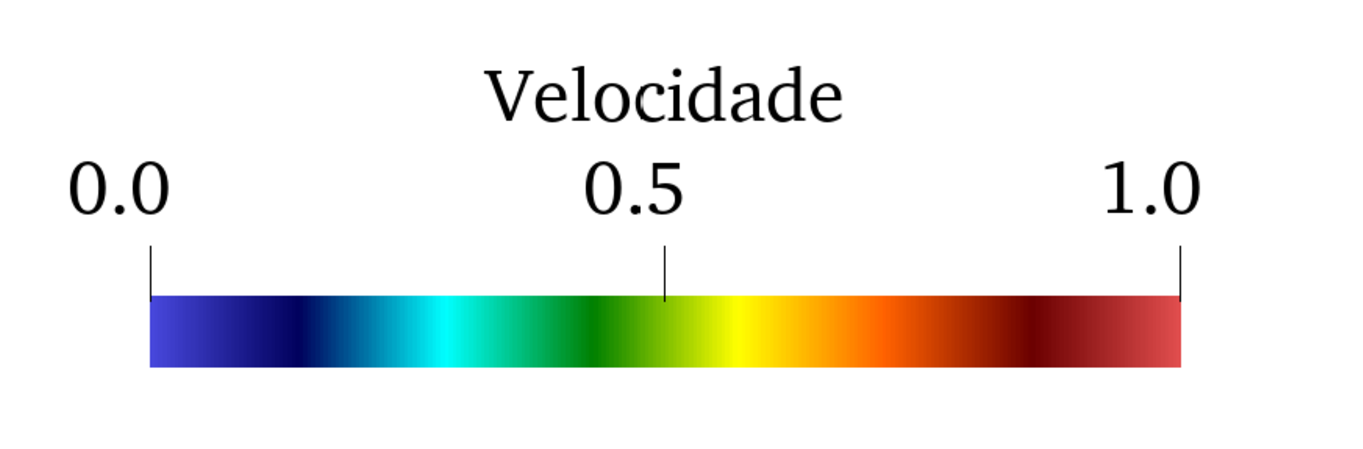
\includegraphics[scale=0.2]{Imagens/Cap2/legandaCavidadeVel.pdf}} 
	\caption{Cavidade quadrada: campos de velocidade. }
	\label{fig:cav3d-vel}
\end{figure}

\begin{figure}[!t]
	\centering
	\setlength{\lineskip}{-10pt}
	\subfloat[\label{fig:cavidade_Press_Re100}$Re$=100.]{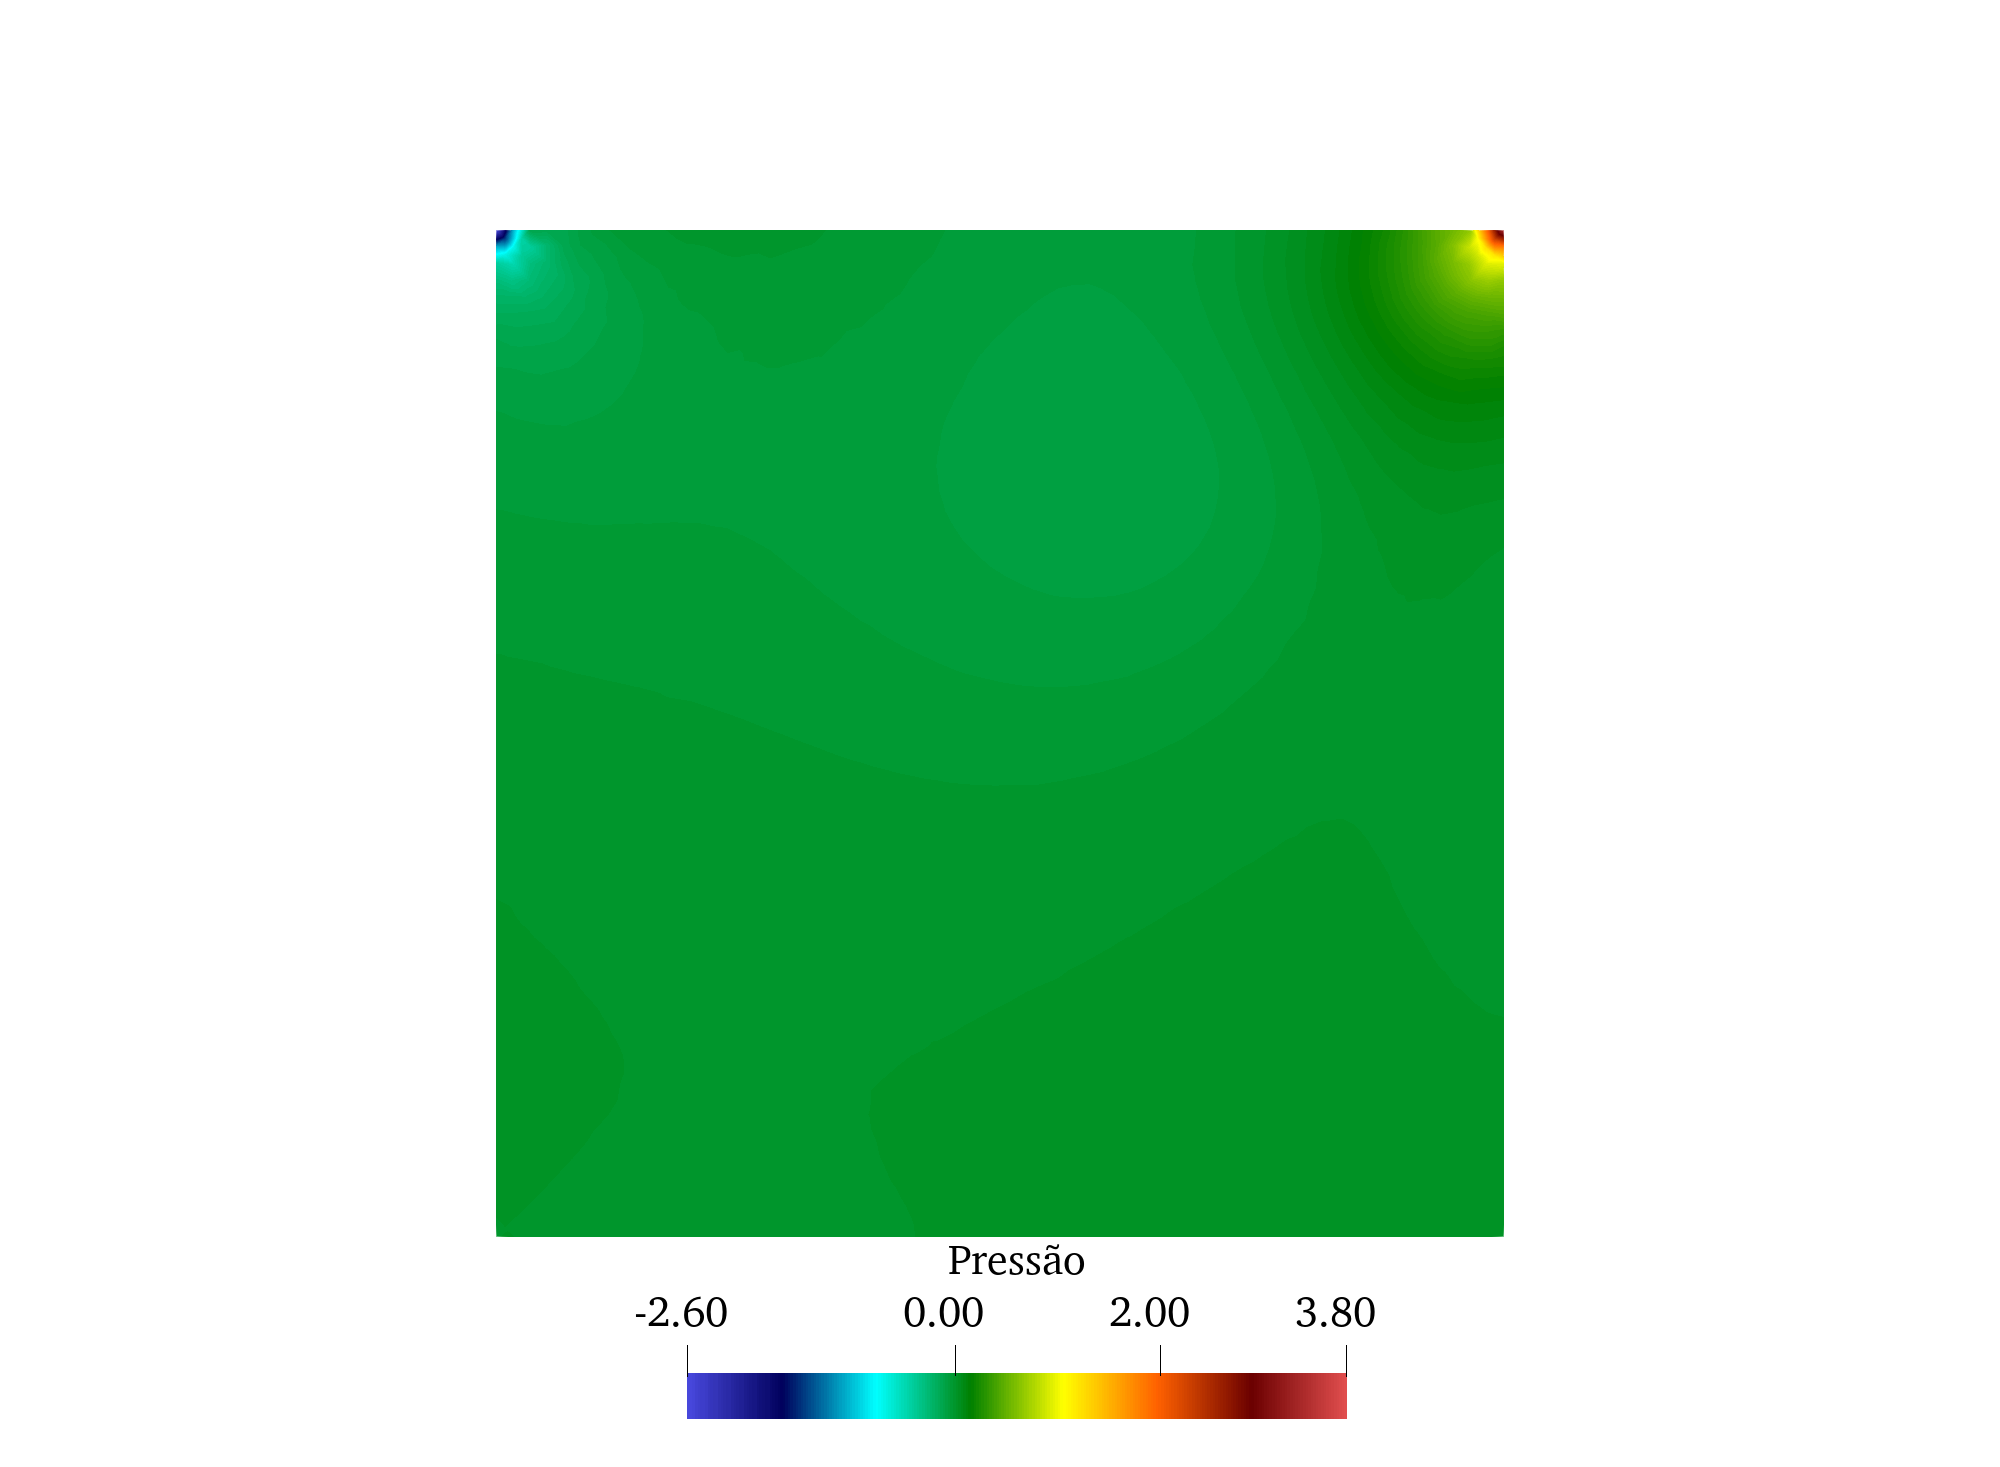
\includegraphics[scale=0.15,trim=15cm 0cm 15cm 7cm, clip=true]{Imagens/Cap2/pressao100.png}} \subfloat[\label{fig:cavidade_Press_Re400}$Re$=400.]{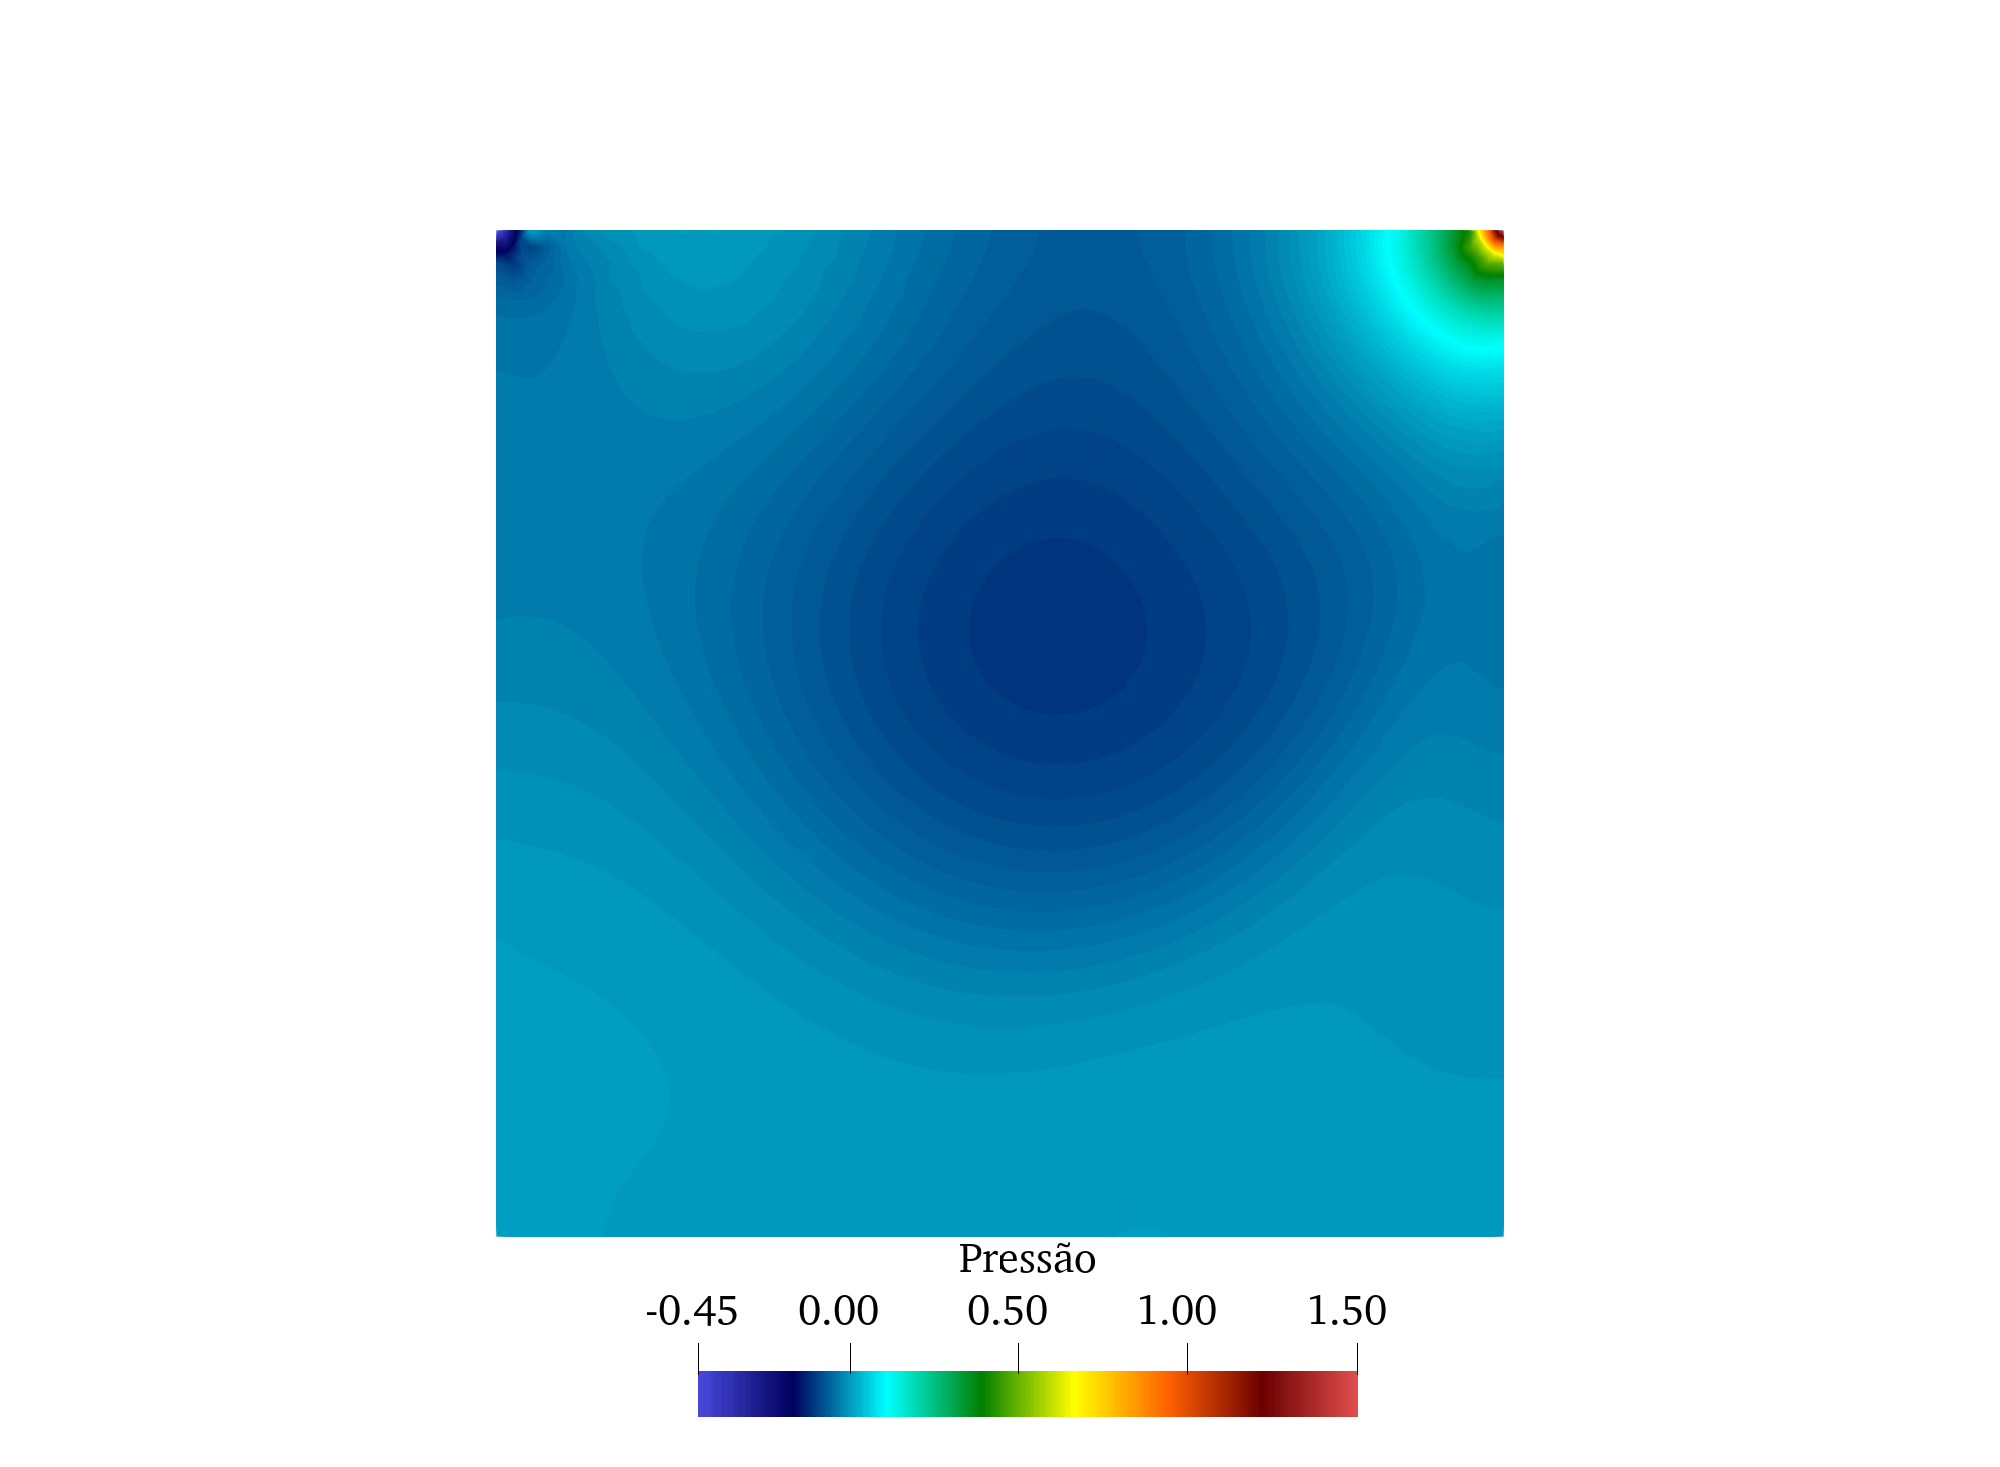
\includegraphics[scale=0.15,trim=15cm 0cm 15cm 7cm, clip=true]{Imagens/Cap2/pressao400.png}}\\ 
	\subfloat[\label{fig:cavidade_Press_Re1000}$Re$=1000.]{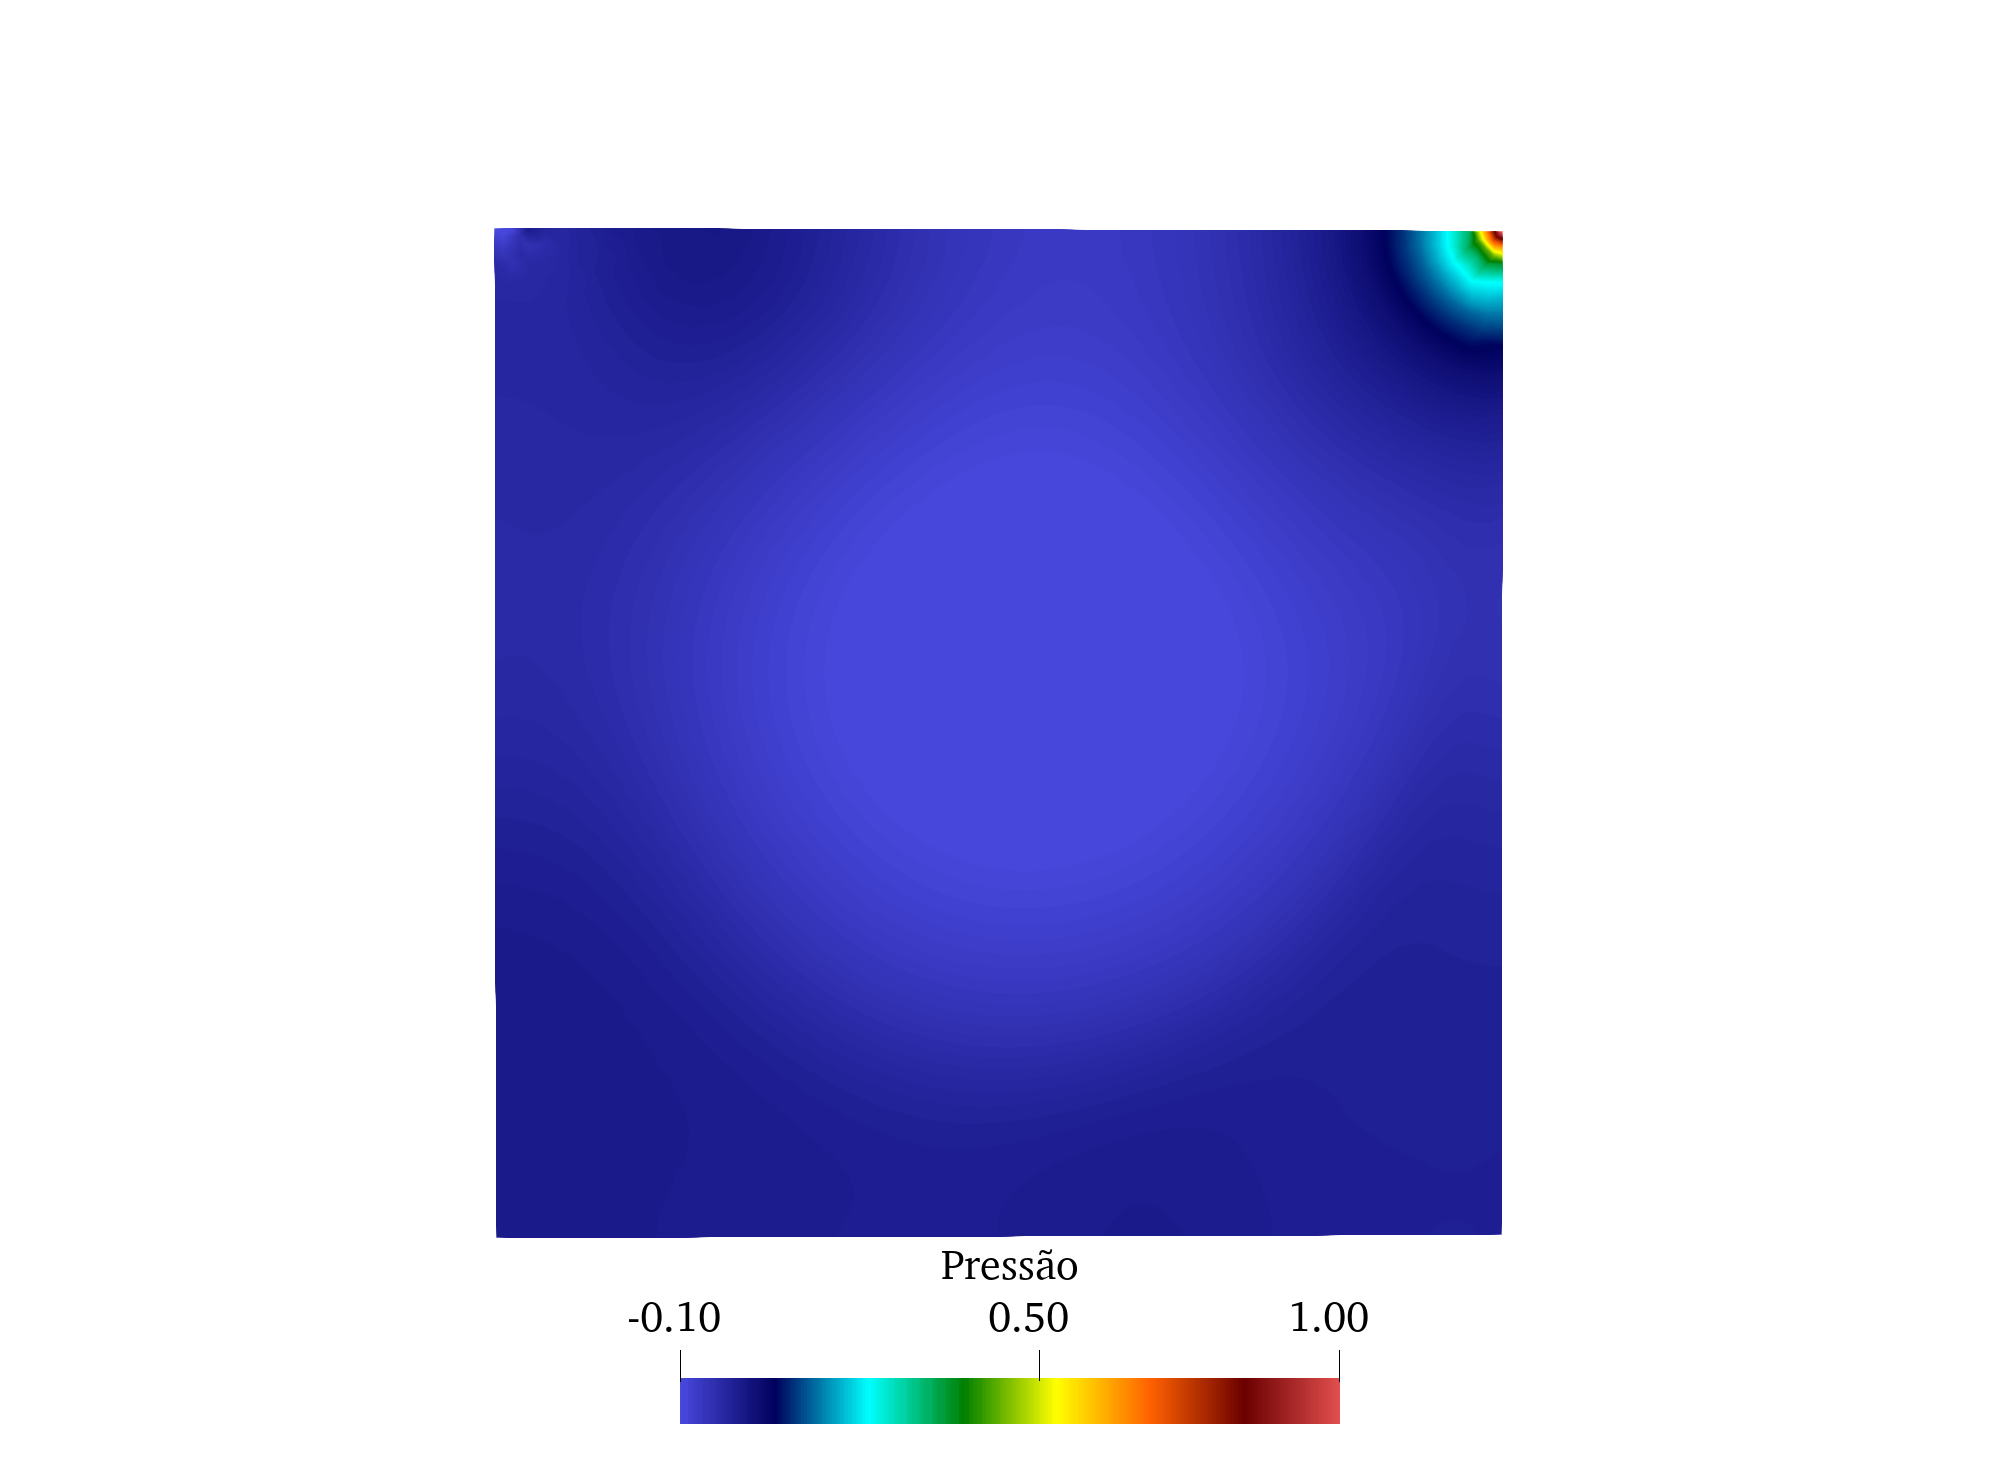
\includegraphics[scale=0.15,trim=15cm 0cm 15cm 7cm, clip=true]{Imagens/Cap2/pressao1000.png}} \\
	%	\subfloat[\label{fig:cavidade_g_Re10000}$Re$=10000.]{\includegraphics[scale=1.1,trim=0.55cm 0.5cm 0.3cm 0.2cm, clip=true]{Imagens/Cap2/cavidade_Re10000.eps}}\\
	\caption{Cavidade quadrada: campos de pressão. }
	\label{fig:cav3d-press}
\end{figure}


%
%\clearpage[e ]
%
%\textcolor{white}{ }


\end{document}
